\documentclass[compress,dvipdfmx]{beamer}

\usepackage[T1]{fontenc}
\usepackage[english]{babel}
\usepackage{lmodern}
\usepackage{beramono}          % Bold in verbatim
\usepackage{hyphenat}          % \hyp{} is a breakable dash
\usepackage{xspace}
\usepackage{graphicx}
\usepackage{alltt}
\usepackage{amssymb,amsmath,stmaryrd}

\newcommand\Inria{\textbf{Inria}\xspace}
\newcommand\Tezos{\textbf{Tezos}\xspace}
\newcommand\Nomadic{\emph{Nomadic Labs (Paris)}\xspace}
\newcommand\FV[1]{\mathcal{F}({#1})}
% Typesetting
%
\newcommand\mypar[1]{\paragraph{#1}\addcontentsline{toc}{subsection}{#1}}
%\newenvironment{sverb}{\small\verbatim}{\endverbatim}
\newenvironment{sverb}{\verbatim}{\endverbatim}

% The TeXbook, Exercise 11.6, p. 311.
%
\def\myfrac#1/#2{\leavevmode\kern.1em
\raise.5ex\hbox{\the\scriptfont0 #1}\kern-.1em
/\kern-.15em\lower.25ex\hbox{\the\scriptfont0 #2}}

% Terms and rules
%
\newcommand\ttcons[2]{{#1}\,$::$\,{#2}}
\newcommand\cons[2]{{#1}\!::\!{#2}}
\newcommand\el{[\,]}
\newcommand\fun[1]{\textsf{#1}}
\newcommand\xkwd[1]{\textsf{\textbf{#1}}}
\newcommand\ufun[1]{\underline{\fun{#1}}}
\newcommand\Lla[1]{\Lleftarrow_{\!{\smash{#1}}}}
\newcommand\Rra[1]{\Rrightarrow_{\!{\smash{#1}}}}

% Languages
%
\newcommand\Coq{\textsf{Rocq}\xspace}
\newcommand\Blang{\textsf{B~language}\xspace}
\newcommand\Simulink{\textsf{Simulink}\xspace}
\newcommand\Lustre{\textsf{Lustre}\xspace}
\newcommand\Esterel{\textsf{Esterel}\xspace}
\newcommand\Promela{\textsf{Promela}\xspace}
\newcommand\UPPAAL{\textsf{UPPAAL}\xspace}
\newcommand\SPIN{\textsf{SPIN}\xspace}
\newcommand\Saxon{\textsf{Saxon}\xspace}
\newcommand\Unicode{\textsf{Unicode}\xspace}
\newcommand\MIME{\textsf{MIME}\xspace}
\newcommand\XML{\textsf{XML}\xspace}
\newcommand\XMLSchema{\textsf{XML Schema}\xspace}
\newcommand\XSLT{\textsf{XSLT}\xspace}
\newcommand\XQuery{\textsf{XQuery}\xspace}
\newcommand\HTML{\textsf{HTML}\xspace}
\newcommand\XHTML{\textsf{XHTML}\xspace}
\newcommand\HTTP{\textsf{HTTP}\xspace}
\newcommand\DTD{\textsf{DTD}\xspace}
\newcommand\Scheme{\textsf{Scheme}\xspace}
\newcommand\XPath{\textsf{XPath}\xspace}
\newcommand\Erlang{\textsf{Erlang}\xspace}
\newcommand\Haskell{\textsf{Haskell}\xspace}
\newcommand\Clean{\textsf{Clean}\xspace}
\newcommand\Prolog{\textsf{Prolog}\xspace}
\newcommand\Java{\textsf{Java}\xspace}
\newcommand\OCaml{\textsf{OCaml}\xspace}
\newcommand{\CamlpF}{\textsf{Camlp4}\xspace}
\newcommand\ocamllex{\textsf{ocamllex}\xspace}
\newcommand\menhir{\textsf{menhir}\xspace}
\newcommand\ocamlyacc{\textsf{ocamlyacc}\xspace}
\newcommand\Ada{\textsf{Ada}\xspace}
\newcommand\Clang{\textsf{C}\xspace}
\newcommand\Michelson{\textsf{Michelson}\xspace}
\newcommand\Fstar{\textsf{F}\(^{*}\)\xspace}
\newcommand\Fsharp{\textsf{F}\(^\sharp\)\xspace}
\newcommand\HACLstar{\textsf{HACL}\(^{*}\)\xspace}
\newcommand\Unix{\textsf{Unix}\xspace}
\newcommand\Cpp{\mbox{\textsf{C} \hspace*{-1.5mm} \raise 0.7mm \hbox
{${\scriptscriptstyle \textsf{++}}$}}\xspace}

% Figures
%
\newcommand\fig{\textsc{figure}}
\newcommand\Fig{\textsc{Figure}}
\newcommand\figs{\textsc{figures}}

% Costs
%
\newcommand\Cost{\mathcal{C}}
\newcommand\Best{\mathcal{B}}
\newcommand\Worst{\mathcal{W}}
\newcommand\Mean{\mathcal{A}}
\newcommand\Trace{\mathcal{T}}
\newcommand\Seq{\mathcal{S}}

\newcommand\C[2]{\Cost_{#2}^{#1}}
\newcommand\B[2]{\Best_{#2}^{#1}}
\newcommand\W[2]{\Worst_{#2}^{#1}}
\newcommand\M[2]{\Mean_{#2}^{#1}}
\newcommand\T[2]{\Trace_{#2}^{#1}}
\newcommand\Call[1]{\Cost\llbracket{#1}\rrbracket}
\newcommand\A[1]{\Seq_{#1}}

\newcommand\Expected[1]{\mathbb{E}[{#1}]}

\newcommand\OC[2]{\OCost_{#2}^{\raisebox{-2.5pt}{$\scriptstyle #1$}}}
\newcommand\OB[2]{\OBest_{#2}^{\raisebox{-2.5pt}{$\scriptstyle #1$}}}
\newcommand\OW[2]{\OWorst_{#2}^{\raisebox{-2.5pt}{$\scriptstyle #1$}}}
\newcommand\OM[2]{\OMean_{#2}^{\raisebox{-2.5pt}{$\scriptstyle #1$}}}
\newcommand\OT[2]{\OTrace_{#2}^{\raisebox{-2.5pt}{$\scriptstyle #1$}}}

\newcommand\OCost{\overline{\Cost}}
\newcommand\OBest{\overline{\Best}}
\newcommand\OWorst{\overline{\Worst}}
\newcommand\OMean{\overline{\Mean}}

% Number-theoretic functions
%
\newcommand\floor[1]{\lfloor{#1}\rfloor}
\newcommand\ceiling[1]{\lceil{#1}\rceil}

% Rewrite systems
%
\newcommand\len[1]{\lvert{#1}\rvert{}}
\newcommand\eqn[1]{\mathrel{\stackrel{\smash{#1}}{=}}}
\newcommand\pair[2]{\langle{#1},{#2}\rangle}
\newcommand\measure[1]{\mathcal{M}\llbracket{#1}\rrbracket}

% Induction
%
\newcommand\total{\succ^t}
\newcommand\predName[1]{\textsf{#1}}
%\newcommand\pred[2]{\predName{#1}\llparenthesis{#2}\rrparenthesis}
\newcommand\pred[2]{\predName{#1}({#2})}

% Word Factoring
%
\newcommand\wlen[1]{\lVert{#1}\rVert{}}
\newcommand\ind[2]{{#1}[{#2}]}
\newcommand\Ind[2]{\ind{#1}{#2}}
\newcommand\BorderName{\mathfrak{B}}
\newcommand\Border[2]{\BorderName^{#1}(#2)}
\newcommand\DBorder[3]{\BorderName_{#1}^{#2}(#3)}
\newcommand\MPfailureName{\mathfrak{F}}
\newcommand\MPfailure[3]{\MPfailureName_{#1}^{#2}(#3)}

\newcommand\prefeqSym{\trianglelefteqslant}    % Prefix
\newcommand\nprefeqSym{\ntrianglelefteqslant}
\newcommand\prefSym{\triangleleft}
\newcommand\nprefSym{\ntriangleleft}

\newcommand\prefeq{\mathrel{\prefeqSym}}
\newcommand\nprefeq{\mathrel{\nprefeqSym}}
\newcommand\pref{\mathrel{\prefSym}}
\newcommand\npref{\mathrel{\nprefSym}}

\newcommand\prefeqName{\mathord{\prefeqSym}}
\newcommand\nprefeqName{\mathord{\nprefeqSym}}
\newcommand\prefName{\mathord{\prefSym}}
\newcommand\nprefName{\mathord{\nprefSym}}

\newcommand\word[1]{\fun{#1}}

% Java keywords
%
\newcommand\abstractX{\texttt{\textbf{abstract}}}
\newcommand\class{\texttt{\textbf{class}}}
\newcommand\extends{\texttt{\textbf{extends}}}
\newcommand\final{\texttt{\textbf{final}}}
\newcommand\main{\texttt{\textbf{main}}}
\newcommand\new{\texttt{\textbf{new}}}
\newcommand\protectedX{\texttt{\textbf{protected}}}
\newcommand\private{\texttt{\textbf{private}}}
\newcommand\public{\texttt{\textbf{public}}}
\newcommand\return{\texttt{\textbf{return}}}
\newcommand\static{\texttt{\textbf{static}}}
\newcommand\super{\texttt{\textbf{super}}}
\newcommand\this{\texttt{\textbf{this}}}
\newcommand\void{\texttt{\textbf{void}}}
\newcommand\nullX{\texttt{\textbf{null}}}
\newcommand\booleanX{\texttt{\textbf{boolean}}}
\newcommand\ifX{\texttt{\textbf{if}}}
\newcommand\elseX{\texttt{\textbf{else}}}
\newcommand\throw{\texttt{\textbf{throw}}}
\newcommand\throws{\texttt{\textbf{throws}}}

% Typesetting Erlang
%
\newcommand\erlcode[1]{\texttt{#1}}
\newcommand\clause[1]{\(#1\)}
\newcommand\smashedrightarrow[1]{\xrightarrow{\smash{#1}}}
\newcommand\smashedleftarrow[1]{\xleftarrow{\smash{#1}}}
\newcommand\MyArrow[2]{\smashedrightarrow{\makebox[#1][c]{\(_\mathrm{#2}\)}}}
\newcommand\fbcode[1]{{\setlength\fboxsep{0mm}\fbox{\phantom{\(\raisebox{-1pt}{#1}\)}}}}
\newcommand\obp{\textbf{(}}
\newcommand\cbp{\textbf{)}}

%% Queues (requires stmaryrd)
%
\newcommand\enq[2]{#1 \mathbin{\Yleft} #2}
\newcommand\deq[2]{#2 \mathbin{\Yright} #1}
\newcommand\emq{\mathord{\circleddash}}

%% Grammars
%
\newcommand\first[1]{\mathcal{P}(#1)}
\newcommand\follow[1]{\mathcal{S}(#1)}

% Beamer configuration
%
\usetheme{default}
\setbeamersize{text margin left=6mm}
\setbeamersize{text margin right=6mm}
\setbeamertemplate{headline}{}
\setbeamertemplate{navigation symbols}{}
\setbeamertemplate{footline}[page number]{}
\setbeamertemplate{itemize items}[circle]
\setbeamertemplate{theorems}[numbered]


\title{Introduction to Formal Methods}
\author{Christian Rinderknecht}
\institute{Eszterházy Károly Katolikus Egyetem}
\date{September 2026}

\begin{document}

\frame{\maketitle}

% ------------------------------------------------------------------------
%
\begin{frame}{Introduction}

  Formal methods are tool-supported methods for software development
  that draw on concepts from theoretical computer science.

  \bigskip

  The reasons for using them are generally:
  \begin{itemize}

    \item reduced maintenance costs (particularly corrective
      maintenance),

    \item robustness (by explicitly delimiting the software's scope of
      validity),

    \item and reliability.

  \end{itemize}

  \bigskip

  Their field of application is therefore, in particular, the
  dependability of critical or embedded systems, since the correctness
  and continuity of service of such systems may put at stake human
  lives or simply large sums of money.

\end{frame}

% ------------------------------------------------------------------------
%
\begin{frame}{Mastering complexity}

  The value of formal methods should not be underestimated.  They have
  required decades of theoretical research as well as experimentation
  and are undergoing rapid expansion.

  \bigskip

  The increase in computing power and the drop in its price \emph{de
  facto} contribute to the relevance of their application and
  sometimes even make their application simply possible in certain
  domains.

  \bigskip

  Some recent advances with AI agents (LeanZip) renew the hope of
  more affordable formal methods.

  \bigskip

  What is at stake here, indirectly, is the mastery of the size and
  logical complexity of computer systems, which is the central theme
  of software engineering.

\end{frame}

% ------------------------------------------------------------------------
%
\begin{frame}{The limits of computing}

  Inventors of perpetual motion machines make us smile because their
  inventions contradict our fundamental knowledge of physics: we know
  \emph{a priori} that there is a flaw without needing to examine the
  details of the mechanism.

  \bigskip

  In computing there are achievements that ought to make us smile
  too. But which ones? Faced with a huge program that \emph{almost}
  works, what should one do?
  \begin{itemize}

    \item Try to complete and correct it so that it works correctly
      and completely?

    \item Reconsider the design and start over with a different method
      for solving the problem?

    \item Conclude with amusement that the problem the program was
      supposed to solve is in fact not solvable by any program, this
      conclusion being drawn without a detailed examination of the
      program?

  \end{itemize}

\end{frame}

% ------------------------------------------------------------------------
%
\begin{frame}{Limits and the engineer}

  Some limits on the use of formal methods are lifted by technical
  progress, but some limits are not due to electronics because they
  are intrinsic to mathematics, and hence to computation. It is thus
  possible to prove that \textbf{certain problems are not solvable and
    never will be}. Knowledge of these extrinsic and inherent limits
  is therefore part of formal methods.

  \bigskip

  Nowadays, the software industry strongly promotes
  pick\hyp{}and\hyp{}choose technologies and parades of
  buzzwords. This is why it is important for the computer engineer to
  understand the foundations of the discipline, which are independent
  of any fashionable technology: this way, he or she will be able to
  correctly \textbf{grasp tools in terms of the concepts} they
  involve.

\end{frame}

% ------------------------------------------------------------------------
%
\begin{frame}{Stakes}

  Public bodies have become aware of the progress made. In Europe (and
  in France since 1995), the ITSEC (\emph{Information Technology
  Security Evaluation Criteria}) require the use of formal methods
  above a certain security level.

  \bigskip

  Along with a broadening of the fields of application (smart cards,
  highly secure information systems, robotics, electronic commerce,
  air traffic control, etc.), requirements have been rising.

  \bigskip

  In certain cases (transportation, control of nuclear power plants,
  medical computing) human lives are at stake.

\end{frame}

% ------------------------------------------------------------------------
%
\begin{frame}{Stakes}

  In telecommunications, the failure of an AT\&T network in January
  1990 caused considerable economic losses.

  \bigskip

  Currently, formal methods are applied to systems ranging from a
  sophisticated algorithm of a few pages to software of several tens
  of thousands of lines, \emph{which is already quite useful}.

  \bigskip

  The explosion of flight~501 of the European Ariane rocket in 1995
  and the failure of a \textsf{Patriot} surface\hyp{}to\hyp{}air
  missile (causing many deaths at a US military camp) are both due to
  software problems and showed the inadequacy of the methods then in
  use in the face of today's challenges.

\end{frame}


\begin{frame}{Complex software is everywhere... and has bugs}

  \begin{center}
    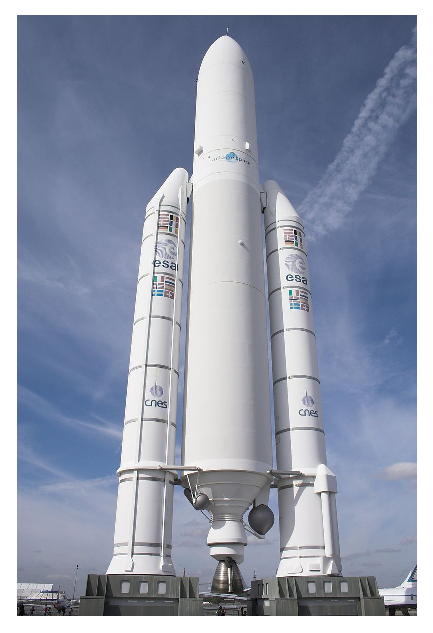
\includegraphics[scale=0.6]{Ariane_5.eps}
  \end{center}

  \centerline{Ariane 5. Credit: ignis, GFDL, CC BY-SA-2.5,2.0,1.0.}

\end{frame}


\begin{frame}{The case of Ariane~5}

  In June 1996, the maiden launch of the European rocket Ariane~5
  ended in its self\hyp{}destruction. The cause was in the software
  controlling the trajectory.

  \bigskip

  This piece of software was designed with the requirements of
  Ariane~4, \textbf{not} Ariane~5. Accordingly, some ranges of
  physical parameters were taken from Ariane~4, and wrongly assumed in
  the programming of Ariane~5.

  \bigskip

  Therefore, certain errors were deemed impossible for physical
  reasons and not handled in the code.

  \bigskip

  During the flight, a value overflowed, causing an exception to be
  raised, but not handled, which lead to the self\hyp{}destruction of
  the rocket (the control system believed that it was off course).

\end{frame}


\begin{frame}{The case of Ariane~5}

  The language used to program that piece of software in Ariane~5 was
  \Ada.

  \bigskip

  \Ada is a programming language originally designed in France in the
  early 80s, before it became the official language for most
  developments for the defence of the USA.

  \bigskip

  \Ada is used a lot in critical embedded systems, deployed in
  transport, aerospace and defence.

  \bigskip

  The language was carefully designed so it lends itself well to all
  sorts of \textbf{static analyses}.

  \bigskip

  These analyses are static because they are performed by the \Ada
  compiler itself, or by other tools that read the source code.

  \bigskip

  Their aim can vary, but perhaps the most important is \textbf{the
    detection of run\hyp{}time errors} before the code is deployed.

\end{frame}


\begin{frame}{The case of Ariane~5 / The after...math}

  The catastrophic failure of the first Ariane~5 incurred a very high
  cost, and the loss of ten years of research and development in
  satellite technology.

  \bigskip

  Some researchers at \Inria (Gonthier \& Deutsch) proposed a static
  analyser for \Ada that could have caught the error that lead to the
  loss of Ariane~5, and discovered many other errors.

  \bigskip

  The mathematical theory they used to analyse the software is called
  \textbf{abstract interpretation}.

  \bigskip

  This powerful theory was invented in the 70s by the French
  researchers Patrick and Radhia Cousot.

\end{frame}


\begin{frame}{PolySpace Technologies}

  In 1999, a start-up company called \textbf{PolySpace Technologies}
  was founded in France by Alain Deutsch (\Inria) and Daniel Pilaud
  (co\hyp{}inventor of \Lustre, a declarative language for programming
  synchronous systems).

  \bigskip

  I joined that company in 2000 to work on the static analysis of
  JavaCard. The idea was to translate JavaCard and other languages
  (\Clang and \Cpp) to \Ada, for which there was already a static
  analyser, following the explosion of Ariane~5. The translation did
  not need to preserve all behaviours, only those who could go wrong
  (run\hyp{}time errors).

  \bigskip

  The company was a success and is now part of \textbf{Mathworks
    Inc.}, known for MATLAB and \Simulink. PolySpace (the tool) is
  well known in the avionics industry.

\end{frame}


\begin{frame}{Abstract interpretation}

  \textbf{Abstract interpretation} is a general framework to analyse
  programs and systems.

  \bigskip

  It makes an \textbf{over\hyp{}approximation} of the behaviours of a
  program, then deduce properties of them, and finally translates back
  the abstract properties in terms of the original behaviours of the
  program.

  \bigskip

  Abstract interpretation is used to replace a system with a possibly
  infinite or very large number of states with a system that has a
  small number of states that can all be checked exhaustively.

  \bigskip

  Abstract interpretation can also be used to \textbf{prove the
    absence of errors}, or to find errors.

\end{frame}


\begin{frame}{Abstract interpretation / An illustration}

  As an illustration, let us consider a system whose states are pairs
  of positive natural numbers, represented as coordinates on a quarter
  of plane.

  \bigskip

  A \textbf{state} is all the information characterising a system
  running at a given point in time: memory contents, program counter,
  files, network buffers, etc. (In the context of functional
  languages, the definition of a state is more restricted.)

  \bigskip

  Some states are coloured in \textcolor{red}{red} to denote that they
  are erroneous: this is the property `To be erroneous'.

  \bigskip

  A behaviour of a system, or \textbf{trace}, can be thought as a line
  from one state to the next. We show four traces as black, thick
  lines. (One of the traces actually ends in an error.)

\end{frame}


\begin{frame}{Abstract interpretation / An illustration}

  \vspace*{15mm}
  \includegraphics[bb=95 428 500 727, scale=0.7]{traces}

\end{frame}


\begin{frame}{Abstract interpretation / An illustration}

  We need to characterise the erroneous states in a simple manner,
  even if we over\hyp{}approximate them: this means to abstract the
  property `To be erroneous.' so it becomes easy to check.

  \bigskip

  For example, we can abstract the error property by a red square
  containing the set of erroneous states, instead of being the exact,
  scattered set itself.

  \bigskip

  A square can be defined by a tiny amount of numbers, and it is easy
  to check whether a given state belongs to it: if so, we deem it an
  error.

  \bigskip

  In our example, this creates \textbf{false positives}, that is,
  states inside the square that are not actual errors.

\end{frame}


\begin{frame}{Abstract interpretation / An illustration}

  \vspace*{15mm}
  \includegraphics[bb=95 428 500 727, scale=0.7]{traces}

\end{frame}

\begin{frame}{Abstract interpretation / An illustration}

  \vspace*{15mm}
  \includegraphics[bb=95 428 500 727, scale=0.7]{traces_square}

\end{frame}

\begin{frame}{Abstract interpretation / An illustration}

  \vspace*{15mm}
  \includegraphics[bb=95 428 500 727, scale=0.7]{traces_square_cropped}

\end{frame}

\begin{frame}{Abstract interpretation / An illustration}

  To reduce the number of false positives, we \textbf{refine the
    abstract property} so it fits better the erroneous states.

  \bigskip

  For instance, we could use another polygon to cover more tightly the
  erroneous states.

  \bigskip

  Let us try an hexagon: to define it, we need the same amount of
  information as for a square, but the inclusion property is slightly
  more complex.

  \bigskip

  This is better, but one trace remains a false positive. In general,
  false positives are inevitable if the property is complex enough, so
  trade\hyp{}offs are necessary.

\end{frame}


\begin{frame}{Abstract interpretation}

  \vspace*{15mm}
  \includegraphics[bb=85 428 500 727, scale=0.7]{traces_square_cropped}

\end{frame}


\begin{frame}{Abstract interpretation}

  \vspace*{15mm}
  \includegraphics[bb=85 428 500 727, scale=0.7]{traces_hexagon}

\end{frame}


\begin{frame}{Astrée}

  \begin{center}
    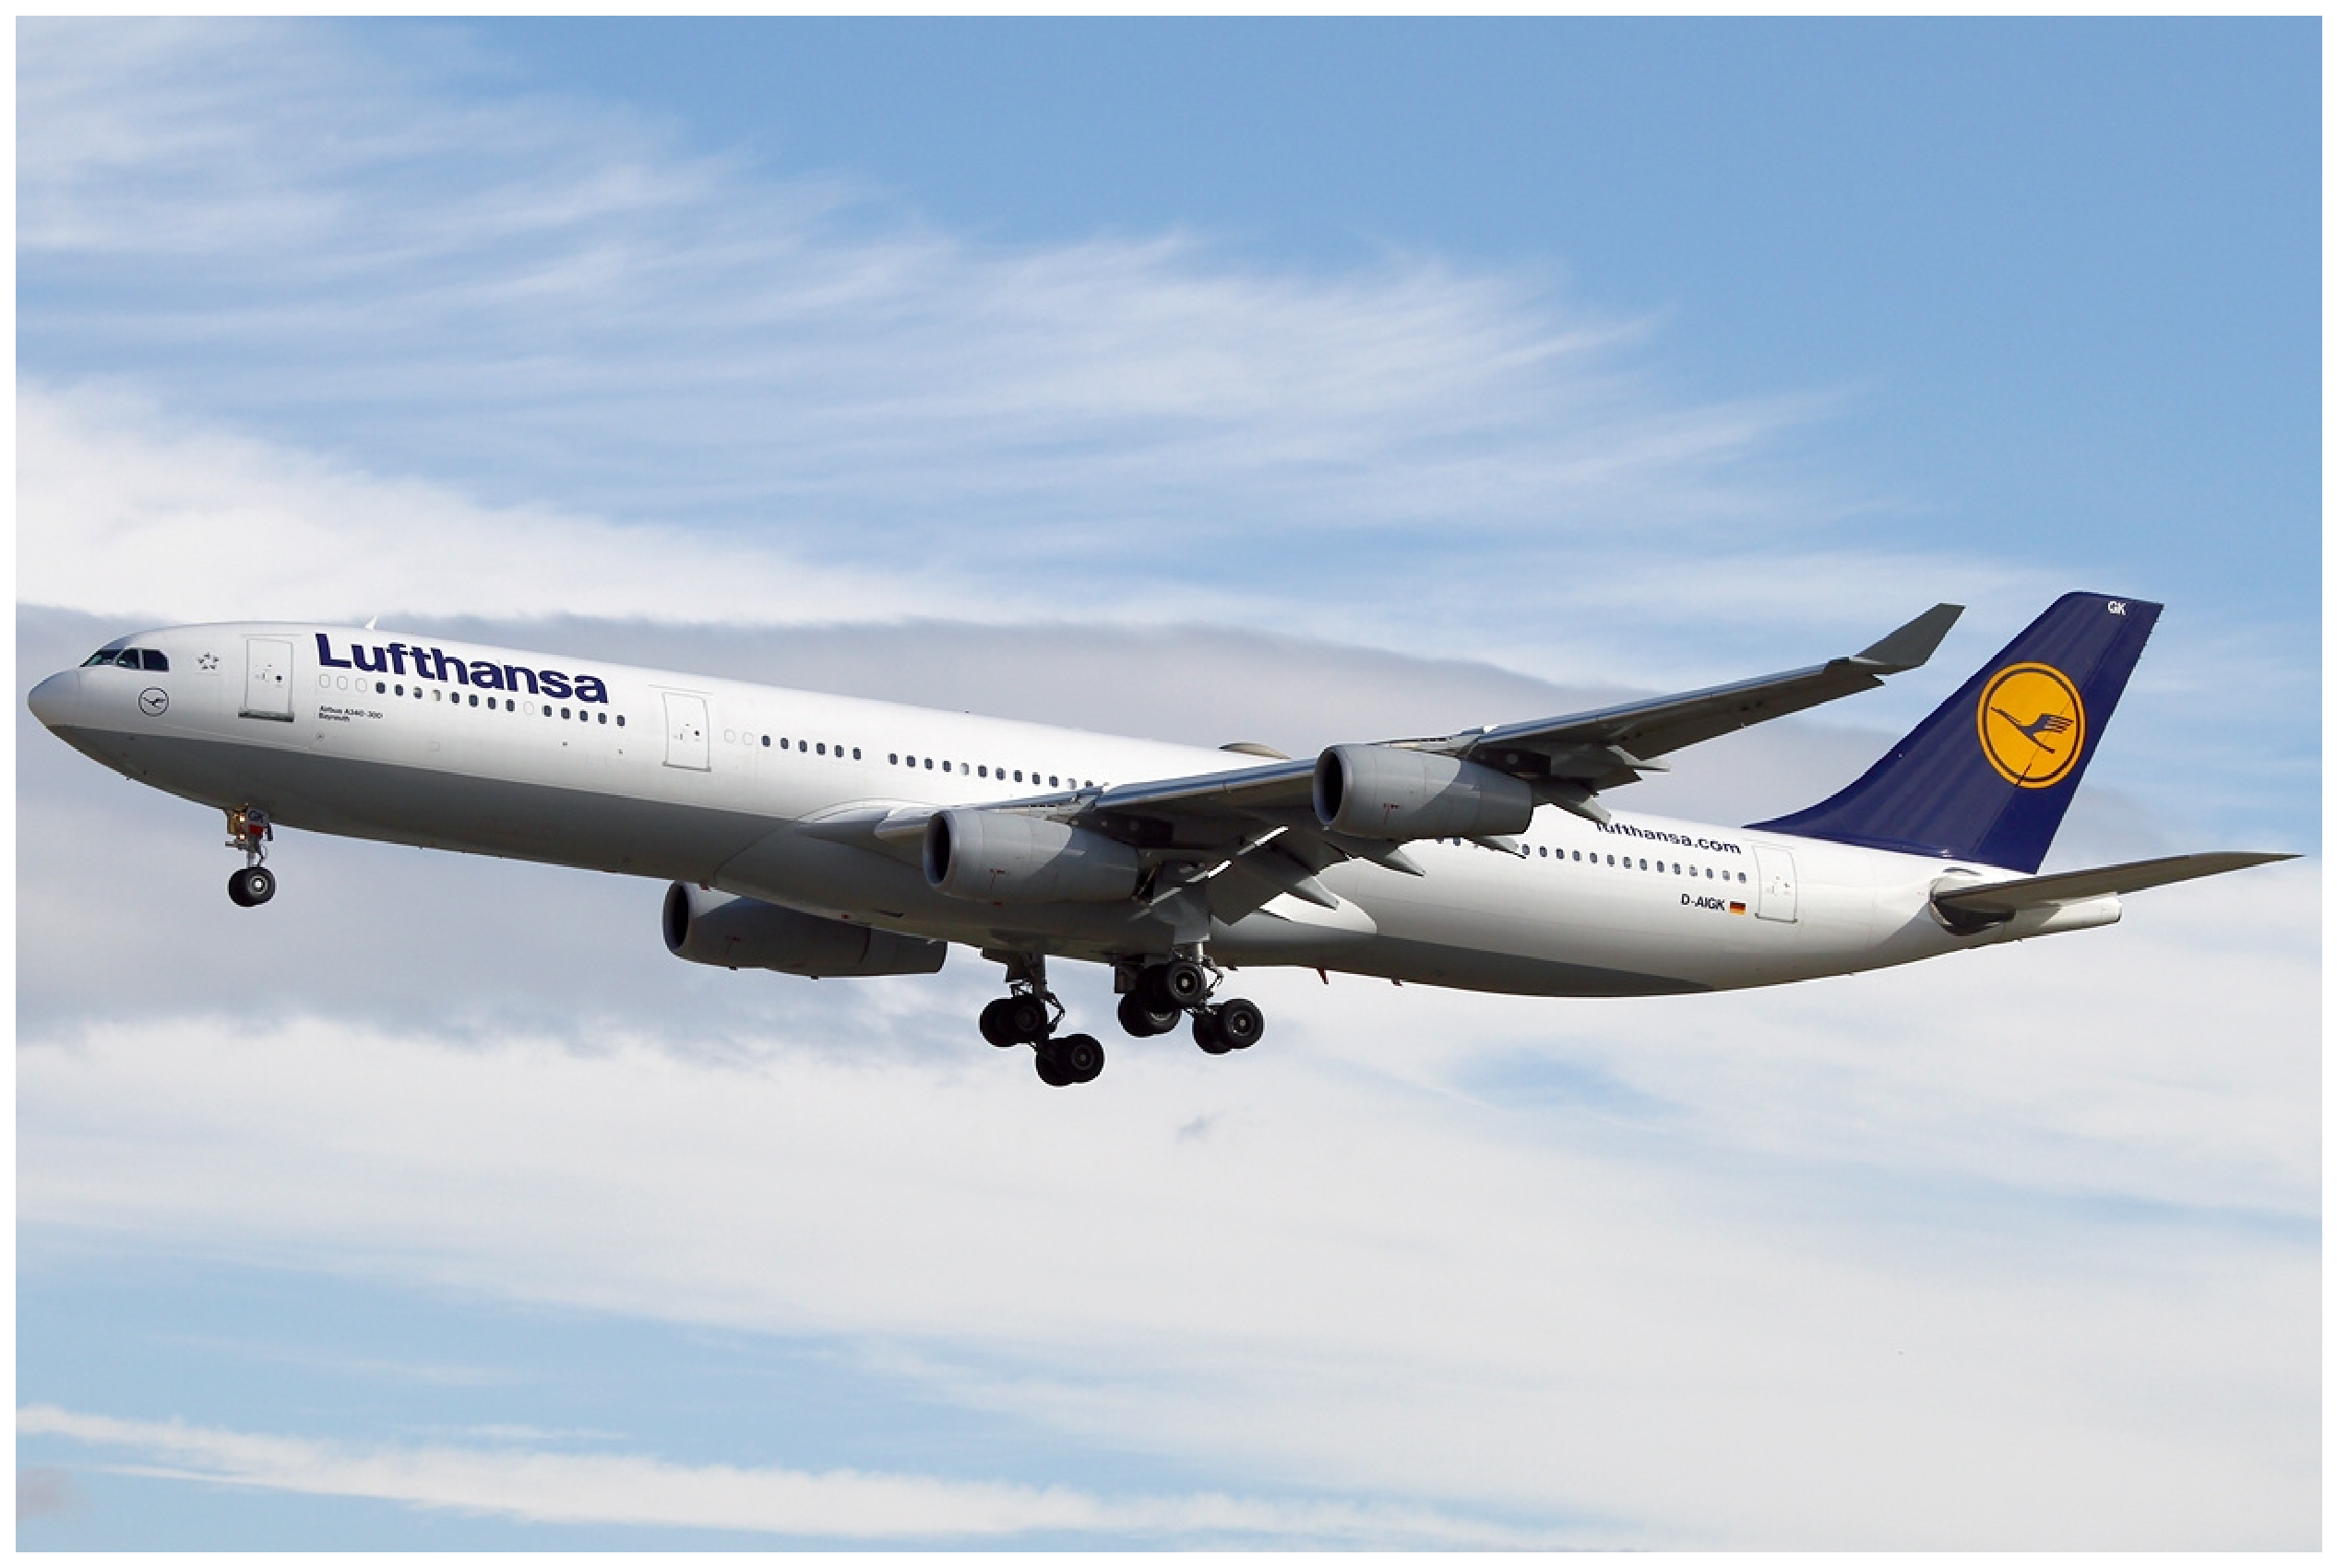
\includegraphics[scale=0.22]{Airbus_A340.eps}
  \end{center}

    \centerline{Airbus A340. Credit: Konstantin von Wedelstardt. GFDL
      1.2}

\end{frame}


\begin{frame}{The static analyser Astrée}

  The usefulness of formal methods should not be underestimated. They
  have taken decades to mature from academic research to practical
  frameworks, and are becoming more and more widespread.

  \bigskip

  \textbf{Astrée} offers an abstract interpretation of \Clang
  programs to detect run\hyp{}time errors, in the same vein as
  PolySpace. It was designed at \'Ecole Normale Supérieure (France)
  and is now commercialised by the German company AbsInt.

  \bigskip

  In 2003, Astrée proved automatically (on a standard PC) the
  absence of any run\hyp{}time errors in the primary flight control
  software of the Airbus A340 fly-by-wire system: 132,000 lines of
  \Clang. Astrée is written in \OCaml and PolySpace in
  \textsf{Standard ML}, the American cousin of \OCaml.

\end{frame}


\begin{frame}{The static analyser Frama-C}

  \begin{center}
    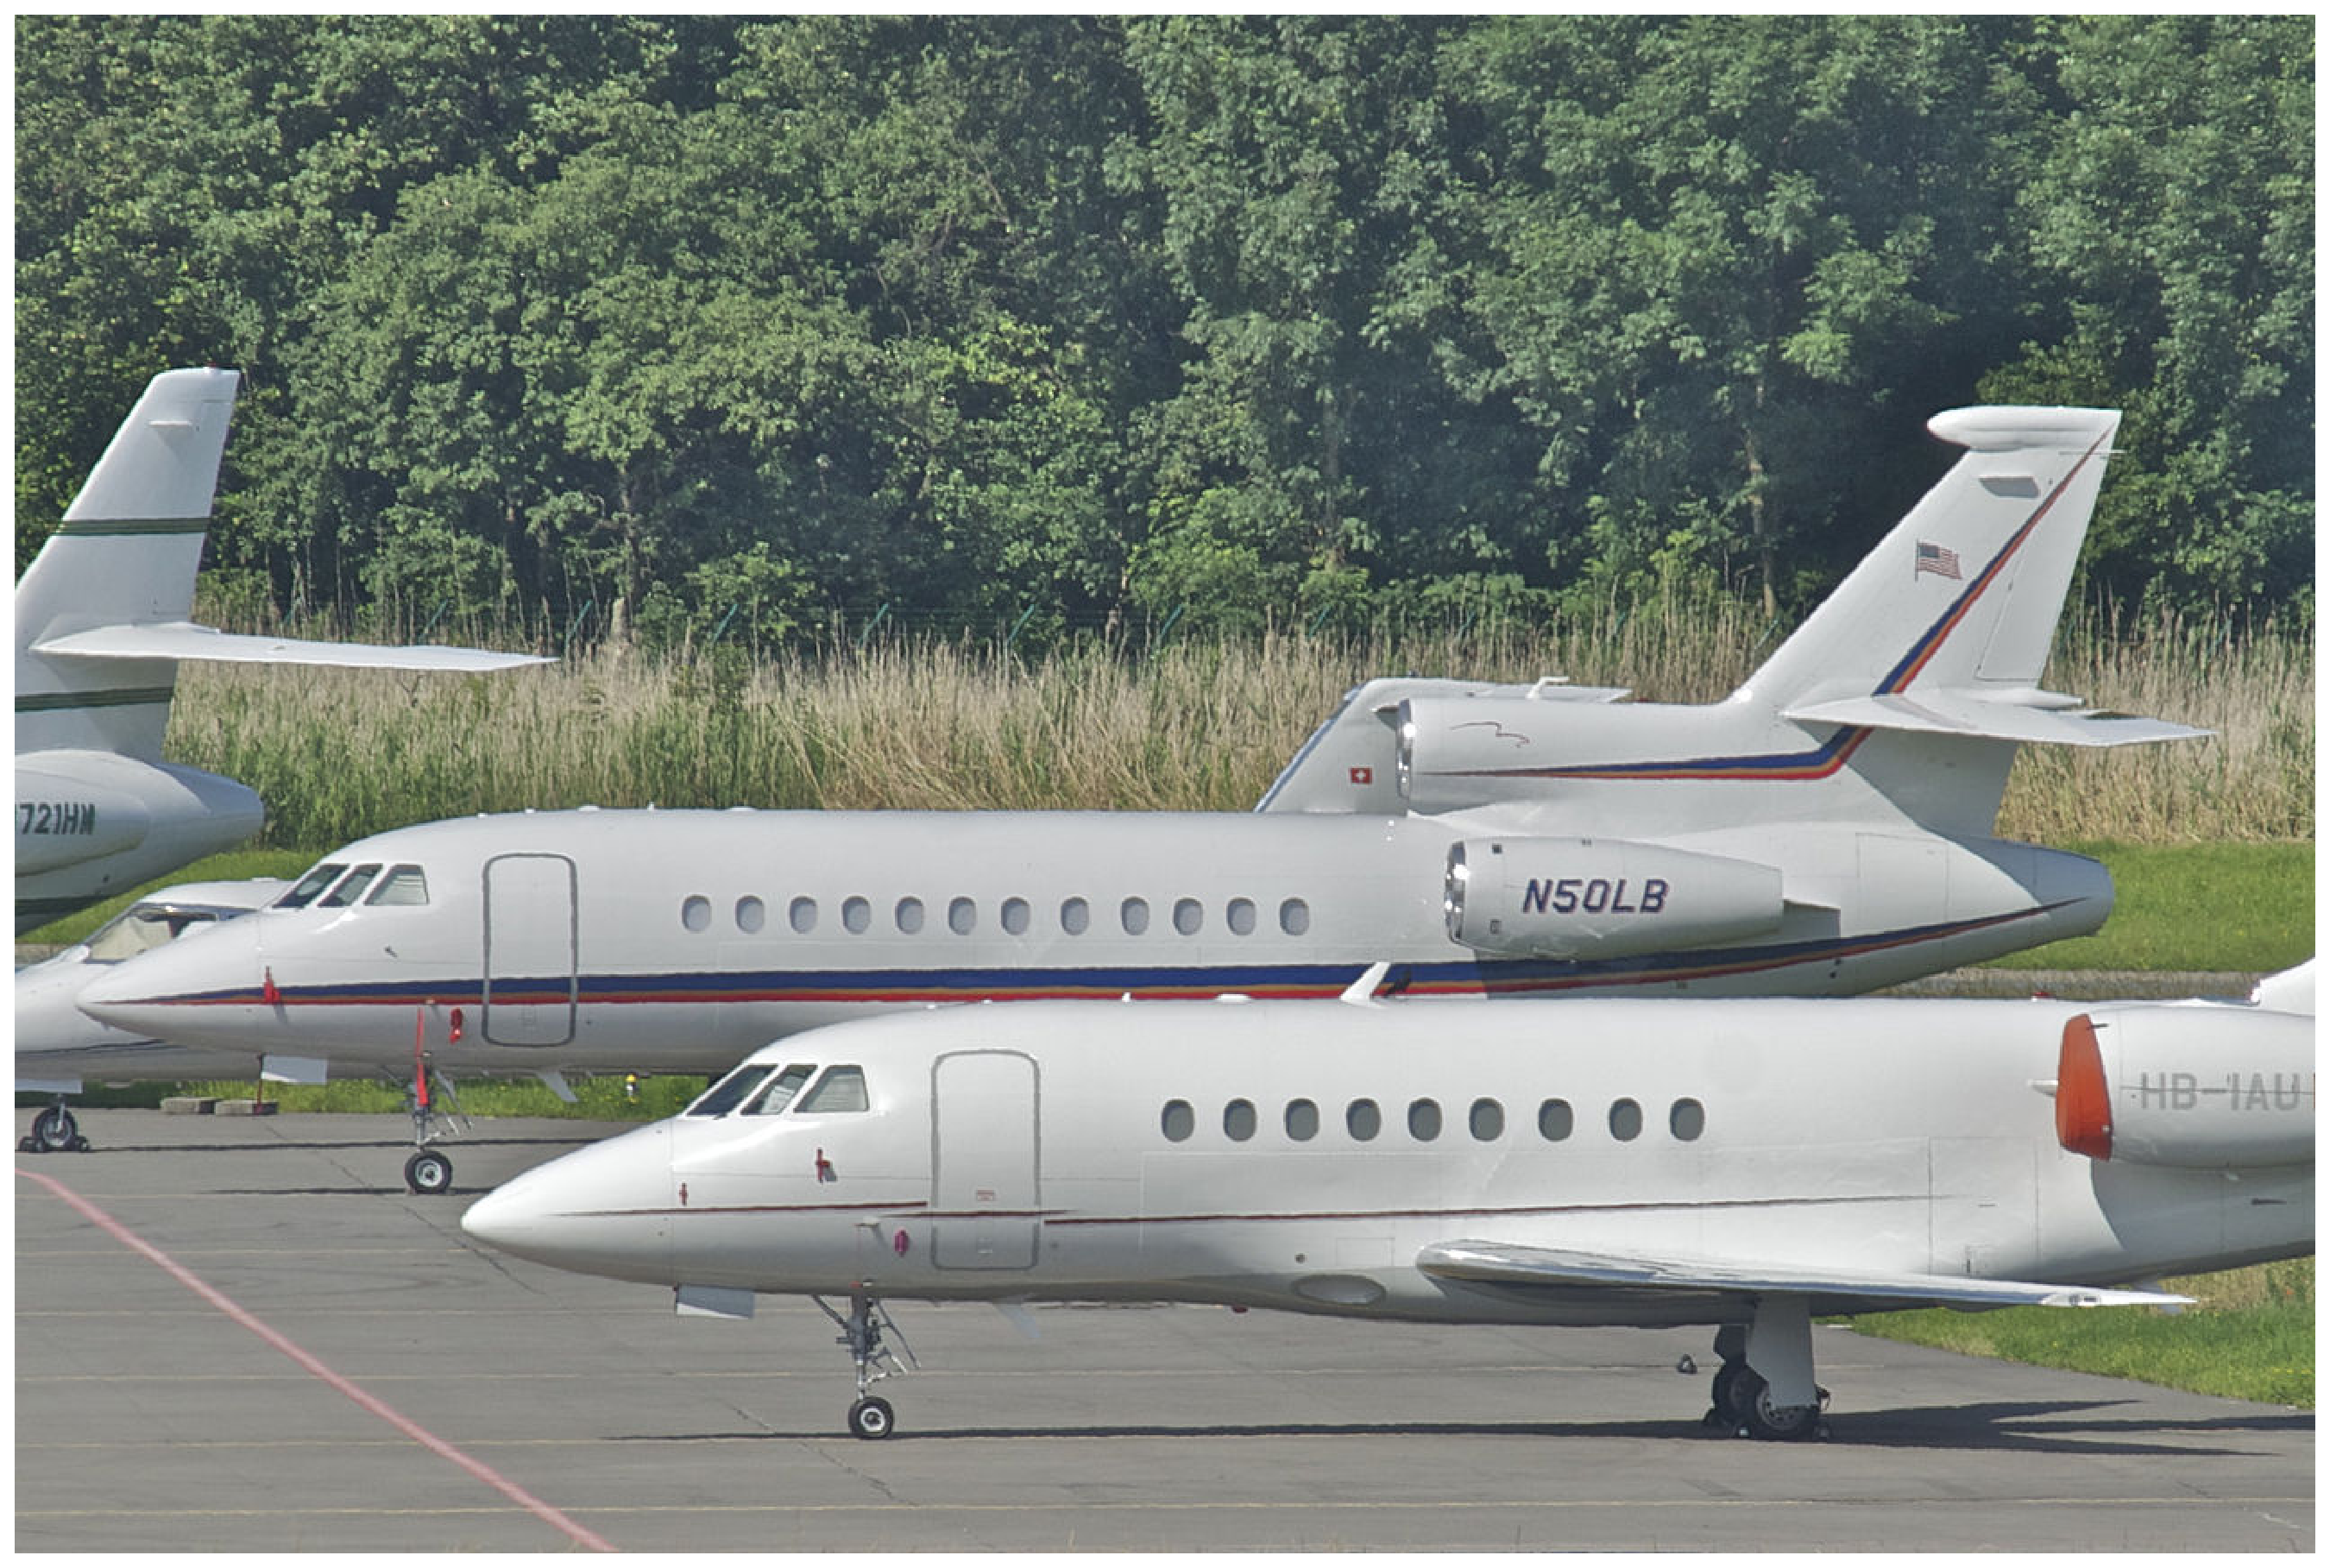
\includegraphics[scale=0.20]{Dassault_Falcon_900.eps}
  \end{center}

  \centerline{Dassault Falcon 900. Credit:  Aero Icarus, CC BY-SA-2.0}

\end{frame}


\begin{frame}{The static analyser Frama-C}

  Another well\hyp{}known static analyser for \Clang is
  \textbf{Frama-C}. It was designed by researchers at the CEA
  (France).

  \bigskip

   Frama-C is actually a software suite which includes a static
   analyser based on abstract interpretation, but also plug\hyp{}ins
   to interactively prove that the source code satisfies some
   \textbf{functional specifications} provided by the user (like model
   checking).

   \bigskip

   Frama-C has been used by Dassault Aviation to detect common
   weaknesses in real\hyp{}time software running on the Falcon jets.

   \bigskip The code base of Frama-C is almost entirely written in
   \OCaml (perhaps the largest \OCaml code base in the world).

\end{frame}


% ------------------------------------------------------------------------
%
%% \begin{frame}
%% \frametitle{Specification for re-engineering}

%% \begin{itemize}

%%   \item An experiment was conducted in 1990 between IBM and the
%%   University of Oxford: a major restructuring of a large transaction
%%   management software system (800,000 lines of assembler and of a
%%   proprietary high-level language).

%%   \item 268,000 lines were modified or rewritten, of which 37,000
%%   were written using the formal method \textsf{Z}. Measurement
%%   facilities were put in place.

%%   \item Development costs decreased by 9\%.

%%   \item During the first eight months following the system's return
%%   to service, customers reported 2.5 times fewer errors in the parts
%%   developed with \textsf{Z} compared with the others, and these
%%   errors were perceived as less severe.

%% \end{itemize}

%% \end{frame}

% ------------------------------------------------------------------------
%
\begin{frame}{Proof of critical railway software}

  To provide strong guarantees of software correctness, one must first
  properly specify the expected behaviour and delimit the scope of the
  proofs.

  \bigskip

  The use of the \textbf{B method} by GEC-Alsthom and, more recently,
  by Matra Transport International for the Calcutta metro (1992) and
  line~14 (1999) of the Paris metro illustrates this approach.

  \bigskip

  This method allows the \textbf{initial specification to be refined
    step by step} and provides a tool (based on set theory) for
  proving at each step the conformity (correctness) of the refinement
  with respect to the previous step. The final phase consists of
  producing several tens of thousands of lines of \textsf{C} code, for
  which one then has, by transitivity, a \textbf{proof of correctness with
  respect to the initial specification}.

\end{frame}


\begin{frame}{A success story: the Parisian metro line~14}

  \begin{center}
    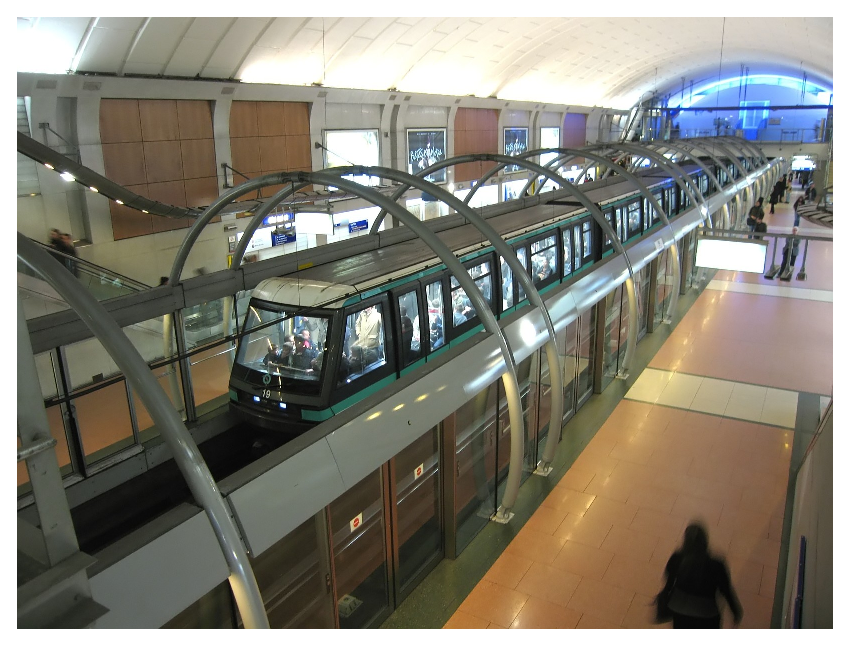
\includegraphics[scale=0.6]{ligne-14-Chatelet.eps}
  \end{center}

  \centerline{Métro line~14. Credit: Pline, CC BY-SA-3.0}

\end{frame}


\begin{frame}{The Parisian metro line~14}

  In October 1999, opened in Paris the first entirely automated metro
  line (number~14).

  \bigskip

  The trains move and stop based on decisions taken by themselves,
  with inputs from sensors and communication networks.

  \bigskip

  To ensure such a high\hyp{}level of safety and continuity of
  service, the company Matra Transport used formal methods from the
  start of the project.

  \bigskip

  After the success of that new metro line, an existing metro line
  (number~1) has been automatised successfully.

  \bigskip

  \textbf{Railways signalling systems} are a major user of formal
  methods, due to the high safety requirements.

\end{frame}


\begin{frame}{The Parisian metro line~14}

  The train system comprises four subsystems:
  \begin{enumerate}
    \item the automatic pilot and signalling system,

    \item the operation control centre,

    \item the platform doors,

    \item the audio-video system.
  \end{enumerate}

  \bigskip

  Only the first  subsystem includes software that is  critical to the
  safety of the passengers.

  \bigskip

  It controls the movement of trains (speed, traction power, routes)
  and the doors (on\hyp{}board and on the platforms).

  \bigskip

  It sends any alarm to the operation control centre.

\end{frame}


\begin{frame}{The Parisian metro line~14}

  The system architecture is naturally distributed and is made of
  \begin{enumerate}

    \item the line equipment, in the operation control centre,

    \item the wayside equipment along the tracks,

    \item the on\hyp{}board equipment.

  \end{enumerate}

  \bigskip

  They are interlinked via a high\hyp{}speed communication network.

\end{frame}


\begin{frame}{The Parisian metro line~14}

  In the operation control centre, operators monitor scheduled train
  programs for each day and supervise events received from the
  network.

  \bigskip

  Platform doors prevent people from falling on the tracks. The train
  doors open only when they are aligned with the platform doors.

  \bigskip

  If not properly aligned, there are emergency doors on the platform
  that can be manually opened.

  \bigskip

  Audio and video feeds allows operators to monitor the inside the
  carriages and to speak with passengers (a high\hyp{}level of
  availability is required to ensure security).

\end{frame}


\begin{frame}{The Parisian metro line~14}

  In order to bring strong correctness assurances in software, it is
  paramount to carefully specify the expected behaviours and delimit
  the scope of the mathematical proofs.

  \bigskip

  The use of the \textbf{B~method} by Matra Transport International
  (now part of Siemens) for the Parisian metro line~14 is a case in
  point of this approach. (Another example is the Calcutta metro, in
  1992.)

  \bigskip

   The B~method was invented in the 80s by Jean-Raymond Abrial, a
   French researcher. It comprises
   \begin{enumerate}

     \item a formal notation to express specifications,

     \item a design methodology,

     \item and software tools.

   \end{enumerate}

\end{frame}


\begin{frame}{The B~method}

  The formal \textbf{\Blang} is based on \textbf{set theory}, which
  makes it very expressive. It enables the specification of a system
  and its expected properties into a model called an \textbf{abstract
    machine}.

  \bigskip

  It also enables the proof of such properties (like safety): some as
  \textbf{system invariants} (properties that must hold on all
  states), some as \textbf{postconditions} to mathematical functions.

  \bigskip

  A \textbf{proof assistant} then either automatically proves some of
  these theorems, or requests the engineer to prove them
  interactively.

  \bigskip

  The B~method and its software tools allow the engineer to
  \textbf{refine} the abstract machine into a series of abstract
  machines until a \textbf{concrete machine} is obtained. A concrete
  machine is one that can be translated automatically into a
  programming language (\Clang or \Ada).

\end{frame}


\begin{frame}{The B~method}

  Each abstract machine is, in turn, less and less
  \textbf{denotational}, and more and more \textbf{operational}.

  \bigskip

   `Operational' means `what a system does', whereas `denotational'
  means `what properties the system satisfies'.

  \bigskip

  Step by step, the abstract machines become closer to
  \textbf{algorithms}, that is, functions operating over data
  structures, which is what a concrete machine is about.

  \bigskip

  The other aspect of a concrete machine is that it is
  \textbf{deterministic}: there are no unspecified choices left in the
  control flow (`what to do next' is always explicit).

\end{frame}


\begin{frame}{The B~method / Refinement}

  \begin{center}
    \includegraphics[bb=71 583 377 721]{refinement}
  \end{center}

\end{frame}


\begin{frame}{The B~language / An abstract machine}

  An abstract machine in the B~language consists of
  \begin{itemize}

    \item \textbf{states}, that is, variables satisfying some
      invariant properties, and

    \item \textbf{operations}, that is, functions that change the
      state while maintaining the invariants, and return values.

  \end{itemize}

  \bigskip

  The variables making up the state of an abstract machine can denote
  mathematical sets, relations, functions, etc.

  \bigskip

  Operations are defined with
  \begin{itemize}

    \item \textbf{preconditions}: `What is assumed about the state by
      the operation before starting', and

    \item \textbf{postconditions}: `What can be assumed about the
      state and return value after the operation is finished'.

  \end{itemize}

\end{frame}


\begin{frame}{The B~language / An abstract machine}

  Let us specify in the B~language what is the Greatest Common Divisor
  (GCD) of two natural numbers.

  \bigskip

  In English: `The GCD of \(x\)~and~\(y\) is~\(d\) such that \(d\)
  divides both \(x\)~and~\(y\), and any divisor of~\(x\) and~\(y\) is
  lower than or equal to~\(d\).'

  \bigskip

  In mathematical notation:
  \begin{equation*}
    \tiny
    \gcd(x,y) \mid x \quad\land\quad
    \gcd(x,y) \mid y \quad\wedge\quad
    \forall z.(z \mid x \;\;\wedge\;\; z \mid y
    \;\; \Rightarrow\;\; z \leqslant \gcd(x,y)).
  \end{equation*}

  The next slide shows the equivalent definition in the B~language
  (note that variables must be at least two characters long).

\end{frame}


\begin{frame}[fragile]
  \frametitle{Greatest Common Divisor (abstract)}

\begin{alltt}
\small
\textbf{MACHINE} gcd /* Greatest Common Divisor */
\textbf{OPERATIONS}
  rr <-- gcd (xx,yy) =
    \textbf{BEGIN}
      \textbf{PRE} xx : INT \& 1 <= xx \& xx < MAXINT
          yy : INT \& 1 <= yy \& yy < MAXINT
      \textbf{THEN}
        \textbf{ANY} dd \textbf{WHERE}
         dd : INT
            \& (xx-(xx/dd)*dd = 0) \& (yy-(yy/dd)*dd = 0)
            \& !zz.(zz : INT \& zz < MAXINT
                   \& (xx-(xx/zz)*zz = 0)
                   \& (yy-(yy/zz)*zz = 0) => zz <= dd)
        \textbf{THEN} rr := dd \textbf{END}
      \textbf{END}
    \textbf{END}
\end{alltt}

\end{frame}


\begin{frame}{The B~method / Refinement}

  The refinement from the initial abstract machine to the final
  concrete machine is stepwise and the engineer must provide more
  details about the low\hyp{}level aspects of the system, whilst
  proving the new specification is \textbf{correct and complete} with
  respect to the previous one (all its behaviours are expected by the
  previous one, and vice\hyp{}versa).

  \bigskip

  This transitively entails that the concrete machine is
  \textbf{equivalent} to the initial abstract machine.

  \bigskip

  The last step consists in the \textbf{generation of \Ada programs}
  (or in \textsf{C}) which are thus, by construction, correct and
  complete with respect to the initial specification.

\end{frame}


\begin{frame}[fragile]
  \frametitle{Greatest Common Divisor (concrete)}

\begin{alltt}
\small
\textbf{REFINEMENT} gcd_R1 /* refinement of ...        */
\textbf{REFINES} gcd       /* ... the previous machine */
\textbf{OPERATIONS}
 rr <-- gcd (xx,yy) = /* No room to handle xx < yy */
   \textbf{BEGIN}
     \textbf{PRE} xx : INT \& 1 <= xx \& xx < MAXINT
         yy : INT \& 1 <= yy \& yy < MAXINT
     \textbf{VAR} rem, old_xx, old_yy \textbf{IN}
     \textbf{WHILE} (yy != 0)
       old_xx := xold_yy := yyrem := xx-(xx/yy)*yy;
       xx := old_yyyy := rem
     \textbf{INVARIANT} gcd (old_xx, old_yy) = gcd (old_yy, rem)
     \textbf{VARIANT} yy < old_yy /* Termination */
     rr := xx
   \textbf{END}
\end{alltt}

\end{frame}

\begin{frame}[fragile]
  \frametitle{The B~language / Ada}

  From the concrete machine, the following \Ada code fragment would be
  produced, were the tooling told to inline the values of the
  variables \texttt{\small rr}, \texttt{\small old\_xx} and
  \texttt{\small old\_yy}, which are only needed for logical reasons
  (to state the invariant and variant, and the final result), not
  computational ones.
\begin{alltt}
\small
\textbf{function} GCD (Xx, Yy : Integer) \textbf{return} Integer \textbf{is}
  Rem : Integer
  \textbf{while} Yy /= 0 \textbf{loop}
    Rem := Xx \textbf{mod} Yy
    Xx := Yy
    Yy := Rem
  \textbf{end loop}
  \textbf{return} Xx
\textbf{end} GCD
\end{alltt}

\end{frame}


\begin{frame}{Formal methods applied to compilers}

  Formal methods can also be applied to \textbf{compilers}.

  \bigskip

  Compilers translate programs of high\hyp{}level languages (`close to
  human thought'), like \Clang, \Ada or \OCaml into programs of
  low\hyp{}level languages (`close to machine thought'), like assembly
  or byte\hyp{}code, and these two programs must be
  \textbf{operationally equivalent}.

  \bigskip

  This means that all behaviours of the input program must be
  preserved in the output program (\textbf{completeness}) and all
  behaviours of the output must map to behaviours of the input
  (\textbf{soundness}, also called \emph{correctness}).

  \bigskip

  Since \Clang is widespread in critical embedded software, it is
  desirable to consider \Clang compilers.

\end{frame}


\begin{frame}{General architecture of a C compiler}

  The compiler is one link in a \textbf{tool chain}:
  \begin{center}
    \includegraphics[bb=71 587 400 721,scale=0.95]{compilation_chain}
  \end{center}

\end{frame}


\begin{frame}{General architecture of a C compiler}

  There are two phases to compilation: \textbf{analysis} and
  \textbf{synthesis}.
  \begin{enumerate}

    \item The analysis breaks up the source program into
      constituent pieces of an intermediary representation of the
      program.

    \item The synthesis constructs the target program from this
      intermediary representation.

  \end{enumerate}

  \medskip

  Actually, there can be many intermediary representations, each one
  getting closer to the target language.

  \bigskip

  Each phase is itself decomposable into other phases, depending on
  the source and target languages.

\end{frame}


\begin{frame}{General architecture of a C compiler}

  The first row makes up the analysis and the second is the synthesis.

  \medskip

  \includegraphics[width=0.9\textwidth]{phases}

  A real compiler is more complex than shown above, and errors are
  likely. Some errors can be silent: some erroneous code can be
  emitted only for certain classes of programs, which is a serious
  problem for embedded applications.

  \bigskip

  Xavier Leroy at \Inria (France) lead the design and implementation
  of a \textbf{certified \Clang compiler}, called \textbf{CompCert},
  using \Coq.

\end{frame}


\begin{frame}{A formally verified C compiler: CompCert}

  CompCert is certified because its \textbf{\OCaml code has been
    extracted from the specification} (of a large subset) of \Clang
  and intermediary representations, as well as from
  \textbf{semantic\hyp{}preserving transformations} between those
  representations, down to optimised assembly.

  \bigskip

  John Regher and his colleagues are experts in finding bugs
  in \Clang compilers. They wrote, in 2011:
  \begin{quote}
    \textit{The striking thing about our CompCert results is that the
      middle\hyp{}end bugs we found in all other compilers are
      absent. [...] This is not for lack of trying: we have devoted
      about six CPU\hyp{}years to the task. The apparent
      unbreakability of CompCert supports a strong argument that
      developing compiler optimisations within a proof framework,
      where safety checks are explicit and machine-checked, has
      tangible benefits for compiler users.}
  \end{quote}

\end{frame}


\begin{frame}{A formally verified C compiler: CompCert}

  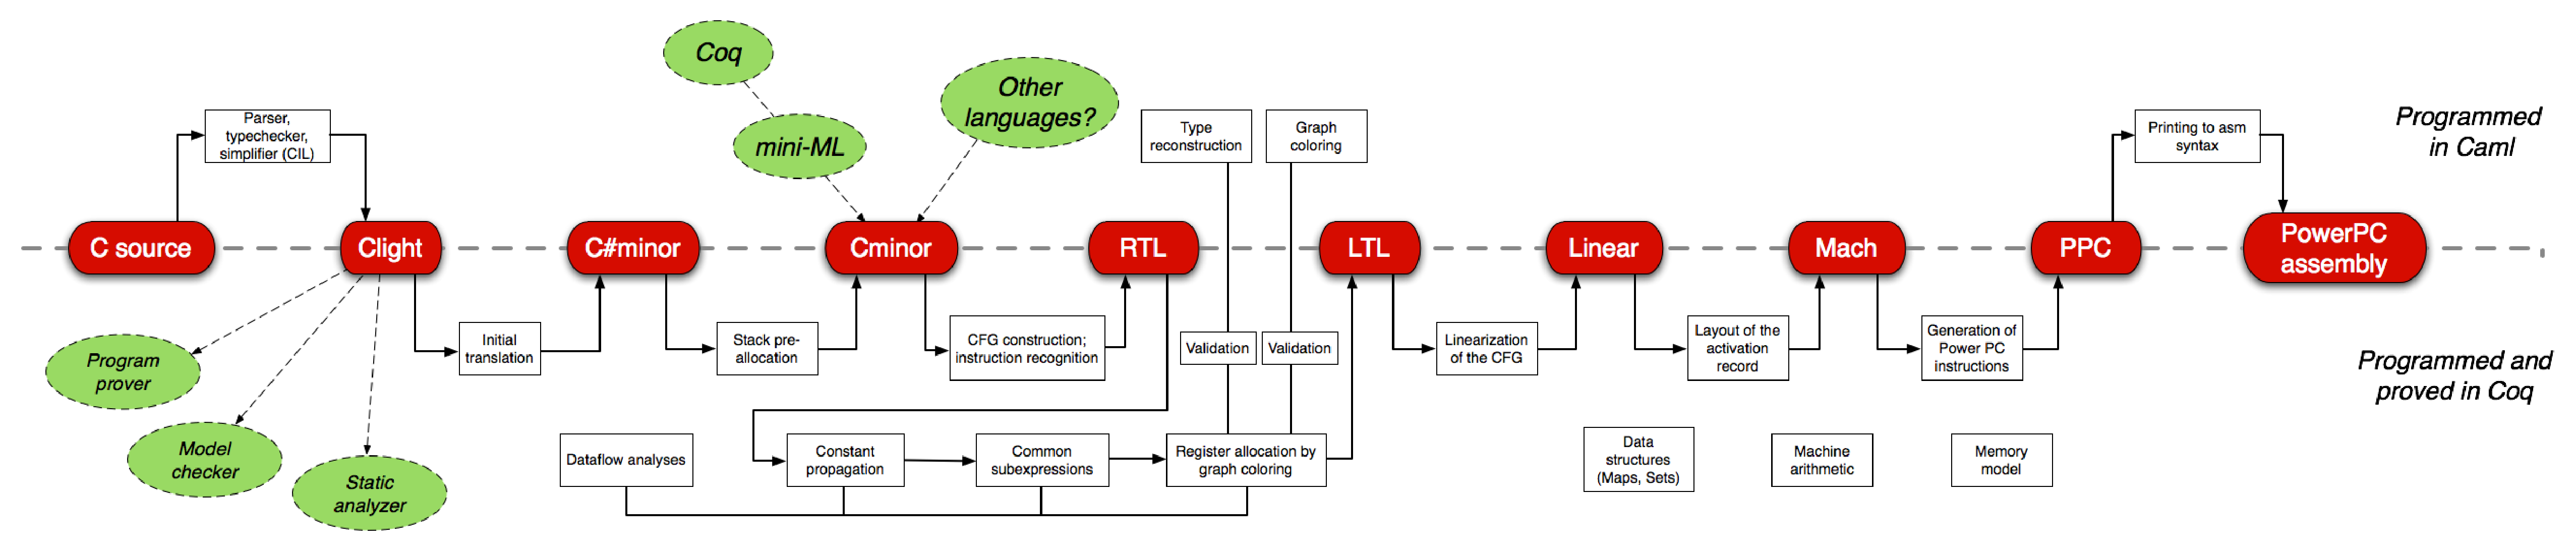
\includegraphics[scale=0.14,angle=35,origin=c]{CompCert_diagram.eps}

\end{frame}


\begin{frame}{The proof assistant \Coq}

  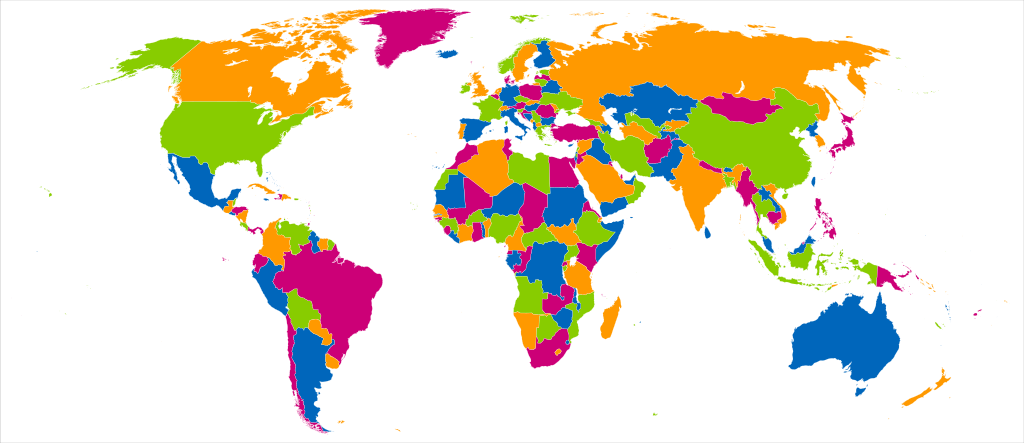
\includegraphics[scale=0.3]{world_map_with_four_colours.png}
  \centerline{Political map of the world. Credit: Fibonacci, CC BY-SA
    3.0}

\end{frame}


\begin{frame}{The proof assistant \Coq}

  \begin{itemize}

    \item \Coq is a \textbf{proof assistant}, that is, a piece of
      software in which to express logical formulas, prove them and
      have the proofs checked automatically. It is an interactive
      tool, but it automates the search of some proof patterns
      (libraries called \textbf{tactics}).

    \item \Coq comes with a programming language named
      \textbf{Gallina} which is close to \OCaml, but \textbf{without
        side\hyp{}effects} and adding \textbf{dependent types}. This
      type system is more general than the type systems found in usual
      languages like \Java.

    \item \Coq features \textbf{code extraction}: it can generate an
      \OCaml program from the proof of its properties.

    %% \item A \textbf{constructive proof} is a proof in which for each
    %%   \(\exists\) quantifier, a witness is given: every object must be
    %%   explicitly built. In particular, this rules out the use of the
    %%   \textbf{law of excluded middle} of classical logic (\(\vdash A
    %%   \lor \neg A\)).

    \item Code extraction relies upon the \textbf{Curry\hyp{}Howard
      correspondence}, which states that a proof is analogous to a
      function, and the proved theorem is analogous to the type of
      that function.

    \item \Coq was created in 1989 by Huet and Coquand, at \Inria
      (France), where it is developed today. It is written in \OCaml.

  \end{itemize}

\end{frame}


\begin{frame}{\Coq: Other Applications}

  Here is a list of compilers certified by \Coq:
  \begin{itemize}

    \item \textsf{CompCert}, an optimising compiler for a subset of C
      by Xavier Leroy in 2012

    \item \textsf{CertiCoq}, a compiler by researchers at Princeton,
      Edinburgh, Inria and Cornell in 2017

    \item \textsf{Q*cert}, a query compiler by IBM Research in 2017

    \item \textsf{Ergo}, a compiler from Ergo (a language of legal
      smart contracts) to \Michelson by Jerôme Siméon in 2018.

  \end{itemize}

   In graph theory, it was used to prove the \textbf{four colour
     theorem}, that states that countries in an arbitrary map can
   always be coloured with four colours (Gonthier, Microsoft Research,
   2008).

\end{frame}


\begin{frame}{Certified cryptographic primitives}

  \begin{center}
    
\includegraphics[scale=0.6]{heartbleed.png}
  \end{center}

  \centerline{Heartbleed bug logo. Credit: Codenomicon, CC0 1.0}

\end{frame}


\begin{frame}{Certified cryptographic primitives / Heartbleed}

  \begin{itemize}

    \item In April 2014 was disclosed a bug in the OpenSSL
      cryptographic library introduced in 2012. The bug was named
      \textbf{Heartbleed} and given a logo to increase public
      awareness.

    \item The bug is due to improper input validation (missing bounds
      check) in the implementation of the TLS heartbeat extension and
      allows protected data to be read.  The bug allows stealing
      private keys and users' session cookies and passwords

    \item The faulty code was written by a PhD student at
      Fachhochschule Münster, and the OpenSSL core developer that
      reviewed the code did not notice the problem.

    \item Around 500,000 SSL certificates were compromised by the bug
      and had to be reissued.

    \item Canada Revenue Agency was stolen 900 social insurance
      numbers in 2014 due to the bug. The records of 4.5 million
      patients were accessed after a breach into the system of
      Community Health, a private hospital in the USA.

  \end{itemize}

\end{frame}


\begin{frame}{Certified cryptographic primitives / HACL*}

  \HACLstar, is a formally verified cryptographic library, developed
  by the Prosecco team at \Inria in collaboration with Microsoft
  Research.

  \bigskip

  \HACLstar is written in \Fstar, an \textsf{ML}-style general-purpose
  functional programming language (with effects) aimed at program
  verification. \Fstar is a cousin of \OCaml and \Coq.

  \bigskip

  The \Fstar code is then extracted into \Clang with the
  \textsf{KreMLin} tool.

  \bigskip

  To generate \Clang code that is proven is correct, the \Fstar code
  is first transformed into \textsf{Low*}, a shallow embedding of a
  subset of \Clang into \Fstar with explicit memory management. The
  code is compiled from \textsf{Low*} to \Clang and compiled with a
  \Clang compiler (certified like CompCert, or not)

\end{frame}


\begin{frame}{Certified cryptographic primitives / HACL*}

  According to the authors of \HACLstar,

  \bigskip

  \begin{quote}
    \textit{when compiled with GCC on 64-bit platforms, our primitives
      are as fast as the fastest pure C implementations in OpenSSL and
      Libsodium, significantly faster than the reference C code in
      TweetNaCl, and between 1.1\(\times\) and 5.7\(\times\) slower
      than the fastest hand-optimised vectorised assembly code [...]}
  \end{quote}

\end{frame}

\begin{frame}{F*}

  \begin{center}
    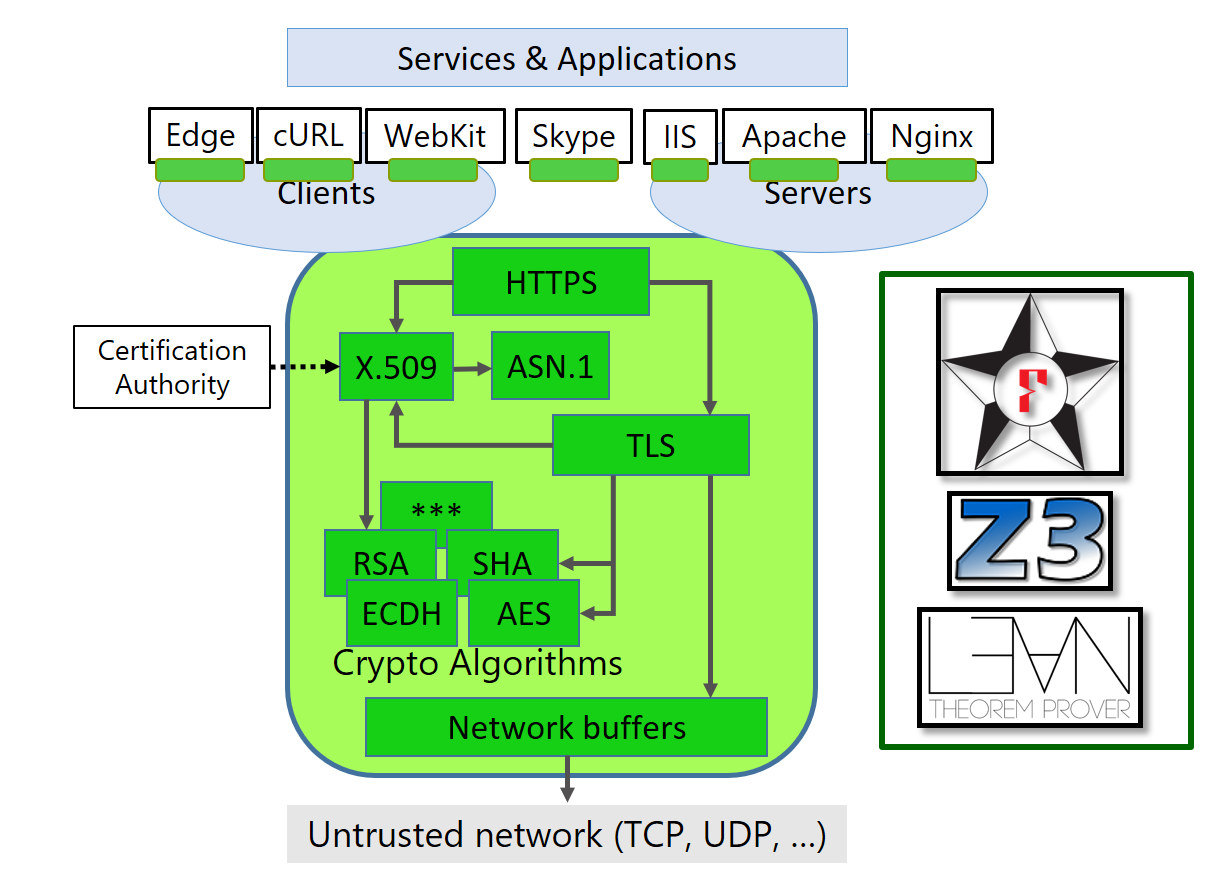
\includegraphics[scale=0.2]{SecureHTTPS.png}
  \end{center}

\end{frame}

\begin{frame}{F*}

  \Fstar is an \textsf{ML}-style general-purpose functional
  programming language with effects aimed at program verification.

  \bigskip

  It was designed and developed at the joint Microsoft Research-Inria
  Centre.

  \bigskip

  \Fstar programs can be extracted to efficient \OCaml, \Fsharp, or
  \Clang code. The \Fstar type-checker aims at proving that programs
  meet their specifications using a combination of \textbf{SMT
    solving} and interactive proofs.

  \bigskip

  Like \Coq, \Fstar can also be helped with intermediate lemmas and
  tactics when it cannot prove automatically the properties of the
  code.

  \bigskip

  There is an online tutorial
  \small\url{https://www.fstar-lang.org/tutorial/}
\end{frame}

%% \begin{frame}
%%   \frametitle{F*}

%%   \begin{center}
%%     \includegraphics[scale=0.12]{InsecureHTTPS.eps}
%%     \includegraphics[scale=0.132]{SecureHTTPS.eps}
%%   \end{center}
%% \end{frame}

\begin{frame}[fragile]
  \frametitle{F*}
   Here is the factorial function in \Fstar:
\begin{alltt}
\small
\textbf{val} fact: n:int\{n \(\geqslant\) 0\} \(\rightarrow\) Tot int

\textbf{let rec} fact n =
  \textbf{match} n \textbf{with}
    0 \(\rightarrow\) 1
  | \_ \(\rightarrow\) n * fact (n-1)
\end{alltt}

The annotation `\texttt{\small n:int\{n \(\geqslant\) 0\}
  \(\rightarrow\) Tot int}' is requesting the \Fstar compiler to prove
that the factorial function terminates (\texttt{\small Tot}) and
returns a positive integer (\texttt{\small \{n \(\geqslant\) 0\}})
when given as input a positive integer.

\end{frame}


\begin{frame}{F*}

  \Fstar proves the function terminates using \textbf{well-founded
    recursion}.

  \bigskip

  If the positivity constraint in the input \texttt{\small n:int\{n
    \(\geqslant\) 0\}} is removed, the type-checker of \Fstar informs
  that it cannot prove the property.

  \bigskip

  Indeed, if \(n < 0\), the function does not terminate and a stack
  overflow occurs.

\end{frame}


\begin{frame}{The Intel Pentium bug}

  \begin{center}
    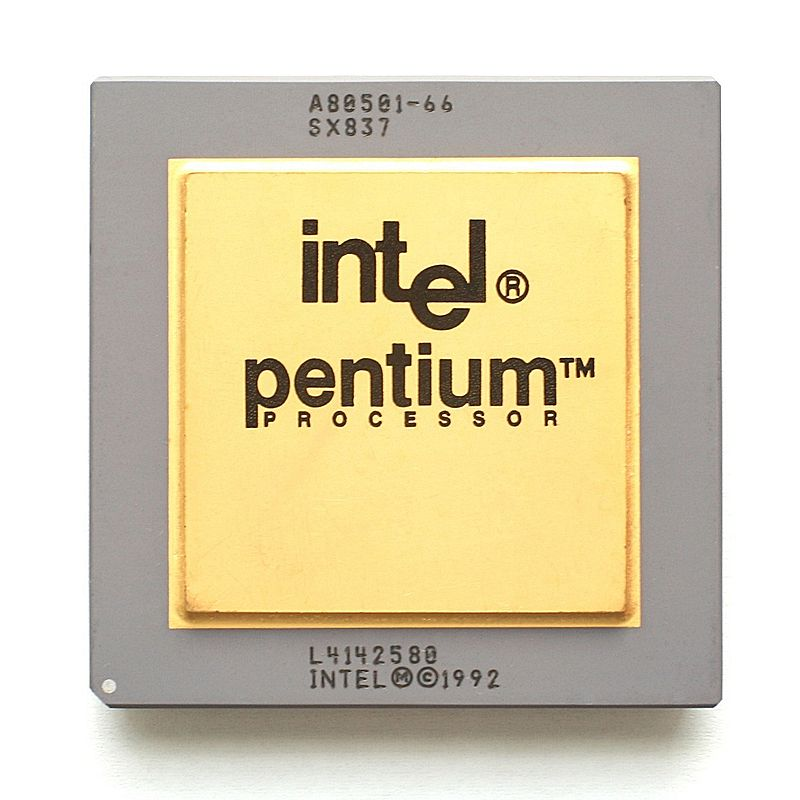
\includegraphics[scale=0.2]{Intel_Pentium_A80501.png}
  \end{center}

  \centerline{CPU Intel Pentium, 66 MHz. Credit: Konstantin Lanzet, CC
    BY-SA 3.0}
\end{frame}

\begin{frame}{The Intel Pentium bug}

  The floating-point unit (FPU) of some Pentium processors (Intel)
  contained an error when a certain kind of division was
  performed. The FPU is a numeric coprocessor, to which the main
  processor (CPU) delegates computations for a speed up (about
  10$\times$).

  \bigskip

  The error was discovered in 1994 by Thomas Nicely, a professor of
  mathematics at Lynchburg College (USA), who was performing
  number\hyp{}theoretic calculations.

  \medskip

  \begin{quote}
    \it The division \(1/824633702441.0\) is calculated incorrectly
    (all digits beyond the eighth significant digit are in error).'
    \\ \hfill ---~Thomas Nicely.
  \end{quote}
  Intel had to recall all faulty units, incurring a large cost, but
  also a very bad press (CNN) in what was at the time a competitive
  market.

\end{frame}


\begin{frame}{The Intel Pentium bug}

  That bug is known as the `Intel Pentium FDIV bug', after the
  instruction for floating\hyp{}point division.

  \bigskip

  Intel reacted by investing in formal methods for the design of its
  chips. For example, John Harrison (Intel) has formally verified the
  correctness (of rounding) of various floating\hyp{}point algorithms
  using the \textbf{HOL Light prover} (a cousin of \Coq, also written
  in \OCaml).

  \bigskip

  Also, various mathematical theorems in elementary number theory and
  real analysis were proved within the same framework.

  \bigskip

  Intel combined theorem proving with a more automated approach when
  the state space is finite and small enough: \textbf{model checking}.

\end{frame}

\begin{frame}{Model checking}

  \textbf{Model checking} was invented in the 80s to check the
  properties of concurrent systems.  (Clarke, Emerson, and Sifakis
  shared the 2007 Turing Award for their work.)

  \bigskip

  Model checking reasons on the \textbf{states of a program}.

  \bigskip

  It requires a way to define
  \begin{itemize}

    \item all possible states of a program, including those that
      should not be reached, and

    \item the execution of a program as the \textbf{transition} from
      one state to another (\textbf{traces}).

  \end{itemize}

  \medskip

  There is usually a very large, but \textbf{finite number of states}.

\end{frame}


\begin{frame}{Model checking}

  \textbf{Temporal logic} is used to express properties of states
  \begin{itemize}

    \item \textbf{Safety}: a given (`bad') state can never be
      reached

    \item \textbf{Liveness}: a given (`good') state will eventually
      be reached

    \item \textbf{Reachability}: a given (`good') state can be
      reached.

  \end{itemize}

  \medskip

  States and sets of states are usually defined with \textbf{logical
    formulas}.

  \bigskip

  \textbf{SMT solvers} are often used to find a trace that leads to an
  undesirable state or prove the state is unreachable by exhausting
  all traces.

\end{frame}


\begin{frame}{Temporal Logic}

  \textbf{Reachability} is a weak property, which is nonetheless useful to
  debug a model under construction, for example, by asserting that a
  process may access a given resource (a scenario can usually be
  automatically constructed).

  \bigskip

  \textbf{Safety} is a strong property reminiscent of a global
  invariant in non\hyp{}temporal logics, and it can be utilised for
  example to state mutual exclusion, that is, that, at any time, there
  will be no more than one process accessing a common resource, or the
  absence of deadlocks, that is, that, at any time, there will be no
  processes waiting transitively on each other for the release of a
  lock on a shared resource.

  \bigskip

  Other interesting safety properties are the non\hyp{}reception of
  unspecified messages and the absence of invalid end states.

\end{frame}


\begin{frame}{Temporal Logic}

  In a temporal logic, doing nothing obviously realises safety, and
  this is where \textbf{liveness} comes into play, to require some
  progress. For example, liveness is useful for expressing the absence
  of starvation, in other words, the fact that a process will gain
  access to a resource.

  \bigskip

  In the theory of programming languages, \textbf{partial
    correctness}, by which, if a program terminates, then its output
  satisfies some condition, would be considered a safety property in
  temporal logics, whilst termination would be considered a liveness
  property.

  \bigskip

  A criterion to distinguish between safety and liveness is the
  following: safety can, in theory, be \emph{disproved} in finite
  time, by simple observation of the states of the system execution,
  whereas liveness can be \emph{proved} in finite time.

\end{frame}


\begin{frame}{Temporal Logic}

  Let us note that temporal logics assume \textbf{infinite futures},
  and since the system is finite, its behaviour must then be
  \textbf{cyclic}, as this happens to be the case of many
  communication systems implementing sessions or interactive loops,
  like servers and command shells.

  \bigskip

  This aspect is perhaps addressed more obviously by properties like
  \textbf{fairness}, which states that `something good will happen an
  arbitrary number of times,' and can be conceived as a repeated
  liveness property. For example: `If access to the critical section
  is infinitely often requested, then access will be granted
  infinitely often.' Fairness is most useful when dealing with the
  scheduling of processes.

\end{frame}

\begin{frame}{The takeaway so far}

  \begin{itemize}

    \item Bugs are everywhere and can be very costly.

    \item The \textbf{B method} helps manually narrowing the gap
      between specification and concrete implementation.

    \item \textbf{Abstract interpretation} runs an approximation of a
      program on an approximation of all possible inputs.

    \item Astrée, PolySpace and Frama-C are abstract interpreters
      written in \OCaml, used in the aerospace industry.

    \item \Coq is a \textbf{proof assistant} used to check
      mathematical theorems.

    \item \Coq is also used to write \textbf{certified compilers}.

  \end{itemize}

\end{frame}

\begin{frame}{The takeaway so far}

  \begin{itemize}

    \item \Fstar enables proving properties of functions using
      \textbf{type annotations}.

    \item \Fstar automatically proves the termination of recursive
      functions using \textbf{well-founded recursion}, but does not
      always succeed.

    \item \Fstar has been used to write efficient certified
      cryptographic libraries.

    \item \textbf{Model checking} is a technique to analyse all
      possible states of a program and prove that some (bad) states
      are unreachable.

    \item States and sets of states are defined with \textbf{logical
      formulas}.

    \item \textbf{SMT solvers} are used to find a trace reaching
      undesired states, or prove the absence of such a trace.

%    \item CubicleW is a model checker written in OCaml, used by Intel
%      to check processor pipeline reordering

  \end{itemize}

\end{frame}

% ------------------------------------------------------------------------
%
\begin{frame}{Communication and rigour}

  An often-overlooked benefit of rigorous or formal semantics is that
  it facilitates \textbf{communication} by providing an unambiguous
  framework for discussion and an impartial arbiter. It is also an
  excellent guide for building support tools (see compilation
  techniques). It is also sometimes possible to state the expected
  properties of a system and even to prove some of them.

  \bigskip

  Let us not forget that software maintenance consumes on average two
  thirds of the total cost of a project, and that fixing a
  specification error requires roughly twenty times more effort if it
  is only detected during operation.

  \bigskip

  Formal methods introduce additional \textbf{rigour} into software
  engineering in order to reduce these costs.

\end{frame}

% ------------------------------------------------------------------------
%
\begin{frame}{In `formal method' there is `method'}

  Software engineering shows that it is important to devote a
  great deal of effort to the early stages of the life cycle and, in
  particular, to establish reliable specifications, that is to say
  \begin{itemize}

    \item ones that correspond well to what is intuitively expected

    \item and that are consistent.

  \end{itemize}

  The first point rests on a good understanding of the client's needs,
  an understanding that the client cannot always articulate from the
  outset.

  \bigskip

  A \textbf{maieutic} process must therefore take place between the
  client and the designer in order to bring out the properties of the
  expected result. The designer builds a formal model step by step,
  which he or she does not necessarily share with the client but whose
  logical implications are discussed with the client in order to
  refine the properties.

\end{frame}

% ------------------------------------------------------------------------
%
\begin{frame}{In `formal method' there is `method'}

  The designer may also resort to \textbf{rapid prototyping}, which
  makes it possible to develop, in a short time, an easily modifiable
  version of the system that appears to be desired. The techniques
  used must then, above all, favour the responsiveness of the
  development process.

  \bigskip

  Considerations relating to the cleanliness or efficiency of the
  software can prove to be a handicap \emph{at this stage}.

  \bigskip

  Once the prototyping stage is complete, priorities change and the
  goals of quality and rigour come back to the fore.

  \bigskip

  The use of functional languages, such as \OCaml, simplifies the
  transition from prototype to product.

\end{frame}

% ------------------------------------------------------------------------
%
\begin{frame}
\frametitle{The formal language as a guiding thread}

  Formulating the problem to be solved in a formal or semi-formal
  language is the first step of the solution. Indeed, a formal
  language can be equipped with a sound semantics, especially if it is
  based on well\hyp{}established mathematical theories.

  \bigskip

  It then becomes possible to prove properties of the system,
  on the one hand at the specification level and, on the other hand,
  at the code level, which can therefore be guaranteed to conform to
  the specification.

  \medskip

  \begin{itemize}

    \item \textbf{Correctness} means that all values returned by the
      program are indeed accounted for by the specification.

      \item \textbf{Completeness} means that the program does not omit
        any of them.

  \end{itemize}

\end{frame}

% ------------------------------------------------------------------------
%
\begin{frame}
\frametitle{The formal language as a guiding thread}

  For reasons that touch on the foundations of mathematics, these
  properties, like others, may not be provable in general (this is
  called \textbf{undecidability}). This brings us back to the limits
  of computability.

  \bigskip

  There are several ways to address conformity (correctness): Hoare
  logic, enumeration of reachable states, refinement of
  specifications, rewriting, program calculation or extraction.

  \bigskip

  A formal language lends itself well to the development of tools that
  automatically assist with the various tasks.

  \bigskip

  Testing, maintenance, and sometimes coding effort are
  reduced, and control over the life cycle increases, as
  documentation becomes much more reliable.

\end{frame}

% ------------------------------------------------------------------------
%
\begin{frame}{Formal methods for the client}

  Formal methods are also relevant to organisations that outsource all
  or part of their software development to third parties. Indeed, the
  client organisation must ensure
  \begin{enumerate}

    \item that its specifications are correct,

    \item that the delivered product matches the specifications.

  \end{enumerate}

  \medskip

  For the second point, the client organisation must, at the very
  least, validate the product and, to do so, subjects it to a battery
  of tests.

  \bigskip

  The complexity of testing grows considerably with that of the
  product and its new versions. Also, automatic generation of test
  suites from formal specifications is achieving increasing success.

\end{frame}

% ------------------------------------------------------------------------
%
\begin{frame}{The limits of testing for the client}

  Testing, while always necessary, can prove insufficient,
  depending on the level of requirements, because it covers only a
  certain number of the system's behaviours. Structural coverage of
  all branches of the code does not account for all possible
  combinations of values (which may in theory be infinite).

  \bigskip

  Sometimes the client organisation supplies the developer with the
  test suite that the product must pass. This can prove problematic if
  the developer deliberately supplies a product that passes the tests
  (a finite number of cases) but is otherwise flawed.

  \bigskip

  If the product is built using formal methods, it can be delivered
  together with a proof of its conformity, which the client
  organisation can then verify. It is far easier to check a proof than
  to discover one.

\end{frame}

% ------------------------------------------------------------------------
%
\begin{frame}{A few caveats...}

  Formal methods are not a panacea: when facing complex problems there
  is no easy solution, only reasoned compromises.

  \bigskip

  One must keep in mind the gap that separates the formal
  specification from the reality it models. This gap can only be
  narrowed through a process of review, reformulation, confrontation
  with conjectures, and maieutic dialogue.

  \bigskip

  One obstacle to the use of formal methods is a lack of mathematical
  culture and familiarity with notation. In civil engineering or
  electronics, mathematics is part of the landscape.

\end{frame}

% ------------------------------------------------------------------------
%
\begin{frame}{... and some good news}

  Formal methods place heavy demands on the early phases of
  development (specification, design), at the risk of giving a
  negative impression of slowdown. But later phases (testing,
  integration) are shortened and better controlled.

  \bigskip

  Formalisation (using logic to model) reveals many tricky points
  earlier. These tricky points are often inherent to the problem to be
  solved, which may therefore be much more complex than it first
  appears.

  \bigskip

  The use of abstract notation is then in fact a plain necessity, not
  an added complication.

\end{frame}

% ------------------------------------------------------------------------
%
\begin{frame}
\frametitle{An overview of formal methods}

Formal approaches present very varied aspects. Several families
currently exist, most of them featuring

\begin{itemize}

  \item a particularly prominent underlying theory (for example,
  transition systems, set theories, universal algebras, the
  $\lambda$-calculus),

  \item a favoured domain of application (for example, data
  processing, real time, protocols)

  \item and a community of researchers and users, sometimes split
  into several variants or schools.

\end{itemize}

\end{frame}

% ------------------------------------------------------------------------
%
\begin{frame}{Specialised or general approaches}

  Specifying a system covers several aspects, including architecture,
  observable behaviours, databases, algorithms, etc.

  \bigskip

  Some methods model systems from the perspective of data
  transformation, or flow, or state machines.

  \bigskip

  Information exchange can be modelled via shared data (centralised
  memory), synchronous communication (which assumes a single clock
  with no propagation delay) or asynchronous messaging, or function
  invocation (of the \emph{Remote Procedure Call} kind in \textsf{C}
  or \emph{Remote Method Invocation} in \textsf{Java}).

\end{frame}

% ------------------------------------------------------------------------
%
\begin{frame}{Specialised or general approaches}

  Other methods are less constraining and provide an excellent general
  interpretive framework.

  \bigskip

  Specialised approaches, by often favouring the operational aspect
  (tooling), can obscure the overall understanding and can struggle to
  keep up with changes to the object being studied.

  \bigskip

  General approaches, closer to mathematical logic, offer great
  freedom of expression but fall short on the methodological front.

\end{frame}

% ------------------------------------------------------------------------
%
\begin{frame}{Example: the role of states}

  A typical example of a difference in approach is the role given to
  the states of a system in its modelling.

  \bigskip

  This notion seems fundamental if one considers the execution support
  of software (computers or virtual machines), which presupposes a
  memory whose contents can change and, possibly, a clock.

  \bigskip

  On the other hand, this notion is not fundamental in mathematics,
  even though mathematics can speak of states. From a theoretical
  standpoint, it is trickier to describe the composition of
  instructions with effects on memory than that of purely mathematical
  functions.

\end{frame}

% ------------------------------------------------------------------------
%
\begin{frame}{Example: the role of states}

  This duality is handled differently depending on the formal
  technique.

  \bigskip

  For example, in the \textsf{B} method there is a notion of
  \textbf{simultaneous assignment}, whose benefit, by grouping a
  sequence of assignments that do not interfere with one another, is
  to reduce the number of states.

  \bigskip

  Moreover, \textbf{functional languages} offer a semantics with no
  notion of state, but also allow states to be used: it is left to the
  programmer to use states (referred to as \textbf{imperative
    features} in programming, such as loops and arrays) only in a
  peripheral way.

\end{frame}

% ------------------------------------------------------------------------
%
\begin{frame}
\frametitle{Favouring specification or verification}
\begin{itemize}

  \item A formal method is built from two main ingredients: a
  specification language and a verification system. These two
  elements are unevenly developed depending on the approach and the
  tools.

  \item Thus, the Boyer-Moore proof-assistance systems favour
  automation of proofs at the expense of ease of expression. In
  contrast, the design of \textsf{Z} aimed above all for expressive
  power, which led to a language that is difficult to tool.

  \item More recent approaches, such as \textsf{HOL} and
  \Coq, try to combine the best of both worlds: relying on
  powerful logics, they come with tools that, on the one hand, help
  construct proofs and, on the other hand, allow those proofs to be
  fully checked with a high degree of confidence.

\end{itemize}

\end{frame}

% ------------------------------------------------------------------------
%
\begin{frame}
\frametitle{Overview of logical tools}

Mathematical logic has developed along several lines:
\begin{itemize}

  \item model theory,

  \item proof theory,

  \item set theory,

  \item type theory,

  \item computability theory.

\end{itemize}
The importance of logic in the context of software engineering can
be summarised in two points:
\begin{itemize}

  \item it provides a framework for expressing many notions;

  \item it lends itself well to formalisation.

\end{itemize}

\end{frame}

% ------------------------------------------------------------------------
%
\begin{frame}
\frametitle{Logic as a framework}

Regarding the first point:
\begin{itemize}

  \item The data manipulated by programs can be described by
    combinations of elementary sets (integers, characters, etc.) such
    as Cartesian products (for \texttt\small {struct} in the
    \textsf{C} language) or unions (for \texttt{\small union} in
    \textsf{C}), for example.

  \item Computability theory teaches us of the existence of limits,
  that is, here, of unrealisable specifications.

  \item Type theory leads to compilers that guarantee the safety of
  programming (through static type checking and inference).

\end{itemize}

\end{frame}

% ------------------------------------------------------------------------
%
\begin{frame}
\frametitle{Logic for modelling}

Regarding the second point, there are two benefits to formalising:
\begin{itemize}

  \item the rigour of texts and reasoning is increased, since they
  can at least partly be reduced to interpretable manipulations of
  symbols;

  \item the resulting work can be assisted or, sometimes,
  automated --- in all cases, tool-supported.

\end{itemize}

\end{frame}

% ------------------------------------------------------------------------
%
\begin{frame}
\frametitle{Model theory}

There are essentially two complementary ways of specifying:
\begin{itemize}

  \item representing a system by its properties,

  \item giving a constructive model of it.

\end{itemize}

This is sometimes referred to as \textbf{specification by properties
  or by models}. Properties are expressed by logical axioms and models
by set\hyp{}theoretic operations. The first case is called the
syntactic aspect and the second the semantic aspect (since it
describes the universe of discourse itself). For example, models
satisfying the statement $\forall x.\exists y.(y \, R \, x)$ include
$(\mathbb{N},>)$ or $(\mathbb{R},<)$ or $(\mathbb{N},\mbox{`is a
  multiple of'})$, etc.

\bigskip

\textbf{Semantic consequence} is fundamental: a statement E is a
semantic consequence of statements A, B, C, etc., if \emph{every}
model having properties A, B, C, etc., also has property E.

\end{frame}

% ------------------------------------------------------------------------
%
\begin{frame}{Proof theory}

  The semantic-consequence relation has the drawback of needing to be
  checked over all possible models, and there may in general be
  infinitely many of them.

  \bigskip

  One may then prefer a \textbf{provability relation}: a statement E
  is said to be provable (or demonstrable) from statements A, B, C,
  etc., if a formal proof of E can be constructed using only the
  hypotheses A, B, C, etc., together with the axioms and rules of
  logic. The statement E is said to be \textbf{refutable} if its
  negation is provable.

  \bigskip

  It is nevertheless necessary that formal manipulations preserve the
  semantics of statements: this is \textbf{soundness}. If every
  semantic consequence is provable, then the theory is said to be
  \textbf{complete}.

\end{frame}

% ------------------------------------------------------------------------
%
\begin{frame}
\frametitle{Proof theory}

Independently of the links between the notions of semantic
consequence and provability, there are questions intrinsic to the
latter, such as: if E is provable, does there exist a proof of E
using only subformulas of E? If so, the search space is
considerably reduced, which has an impact on proof assistance.

\bigskip

The study of axioms and rules as formal (that is, purely syntactic)
calculi, together with their relationships to the notion of semantic
consequence, constitutes \textbf{proof theory}.

\end{frame}

% ------------------------------------------------------------------------
%
\begin{frame}
\frametitle{Cantor's set theory and Russell's paradox}

It is useful to form a set whose elements possess a given
property --- such a definition is said to be \emph{by
  comprehension}. If this type of definition is left unconstrained,
one ends up within the framework of the first, so-called naive, set
theory, which turned out to be contradictory at the beginning of the
20th century.

\bigskip

A theory is contradictory if one can prove both a statement and its
negation, and hence, in the end, anything at all.

\bigskip

Consider Russell's paradox. Let us form, by comprehension, the
curious set $R = \{x \mid \neg(x \in x)\}$. If $R \in R$ then $R$
must satisfy the property held by its elements, namely $\neg(R \in
R)$. Conversely, if $\neg(R \in R)$ then $R$ satisfies the defining
property of the elements of $R$, that is, $R \in R$. Hence, setting
the property $P = R \in R$, we have proven both $P$ and $\neg{P}$,
which is contradictory.

\end{frame}

% ------------------------------------------------------------------------
%
\begin{frame}
\frametitle{Zermelo-Fraenkel axiomatic set theory}

One way to circumvent the pitfall of paradoxes is to reformulate set
theory axiomatically (that is, with logical rules) by introducing a
form of \emph{stratification of constructions}. In this way, a
property cannot be arbitrarily defined by ranging over an arbitrary
property, as is the case in Russell's paradox.

\bigskip

This theory, proposed by Zermelo and Fraenkel, allowed for a
new foundation of mathematics, and no one has reproduced a paradox
within it to this day.

\bigskip

The specification languages \textsf{Z} and \textsf{B} rely on this
theory, adding a touch of typing to bring it closer to the concerns
of computer science.

\end{frame}

% ------------------------------------------------------------------------
%
\begin{frame}
\frametitle{Type theory}

Another way to avoid paradoxes was proposed by Russell himself: type
theory. This too involves stratifying sets (and properties): at
level~0, individuals; at level~1, sets of individuals (and
properties concerning individuals); at level~2, sets of sets of
individuals, and so on. Types characterise these layers. They are
associated with individuals and with basic properties and constrain
the construction of the higher layers.

\bigskip

In computer science, this approach has proven very fruitful, as
shown by many recent programming languages. To allow for recursion,
a more permissive typing rule is needed. The unavoidable drawback is
then having to allow programs that do not terminate.

\end{frame}

% ------------------------------------------------------------------------
%
\begin{frame}
\frametitle{Computability theory}

Another fundamental aspect is the question of which mathematical
functions are computable by machines: this is the subject of
computability theory.

\bigskip

In the 1940s, several approaches were proposed:
\begin{itemize}

  \item Turing machines,

  \item the $\lambda$-calculus (Church),

  \item partial recursive functions (Gödel, Herbrand).

\end{itemize}
Each provides a framework in which to express a notion of
\emph{effective procedure} (algorithm). The \emph{Church thesis} is
that these various formalisms are equivalent (they compute the same
set of mathematical functions).

\end{frame}

% ------------------------------------------------------------------------
%
\begin{frame}
\frametitle{Countable sets}

Are all functions computable? To answer this, a detour through the
theory of formal languages proves useful.

\bigskip

A set is \emph{countable} if it is finite or can be put in
bijection with the set of natural numbers $\mathbb{N}$. The
cardinality of a countably infinite set is denoted $\aleph_0$. For
example
\begin{itemize}

  \item The set of even numbers is countable (the trivial bijection
  is $2n \mapsto n$). In general, every infinite subset of the
  naturals is countable.

  \item The set of finite words over the alphabet $\{a,b\}$ is
  countable (the bijection is built by ordering the words
  lexicographically).

  \item The rational numbers are countable.

  \item Regular expressions are countable.

\end{itemize}

\end{frame}

% ------------------------------------------------------------------------
%
\begin{frame}
\frametitle{Cantor's diagonalisation}

One may then ask whether there exist sets whose cardinality is greater
than $\aleph_0$, that is uncountable sets. The answer is yes:
\textbf{the set of subsets of a countable set is not countable.}

\bigskip

This is proven by a technique called \textbf{diagonalisation}. Let $A
= \{a_0, a_1, \ldots\}$ be a countable set and let $S$ be the set of
its subsets.

\bigskip

Let us argue by contradiction and assume that $S$ is countable, and
therefore that $S = \{s_0, s_1, \ldots\}$.

\end{frame}

% ------------------------------------------------------------------------
%
\begin{frame}
\frametitle{Cantor's diagonalisation}

Let us construct the following infinite table:
\[
\begin{array}{c|cccccc}
       & a_0    & a_1    & a_2    & a_3   & a_4      & \ldots\\
\hline
s_0    & \times & \times &        & \times \\
s_1    & \times & \circ  &        & \times \\
s_2    &        & \times & \times &        & \times\\
s_3    & \times &        & \times & \circ  & \\
s_4    &        & \times &        & \times & \circ\\
\vdots &        &        &        &        &         & \ddots
\end{array}
\]
It indicates which elements of $A$ belong to which elements of $S$:
a cross at column $i$ and row $j$ indicates that $a_i \in s_j$.

\end{frame}

% ------------------------------------------------------------------------
%
\begin{frame}
\frametitle{Cantor's diagonalisation}

Consider the set $D = \{a_i \mid \neg(a_i \in s_i)\}$. Its elements
are marked with a circle in our table (on the diagonal). We have
$D \subset A$, but is $D$ actually listed among the $s_j$?

\bigskip

Suppose there exists $k$ such that $D = s_k$. But $a_k \in D
\Leftrightarrow \neg(a_k \in s_k)$, which implies $D \neq s_k$,
thus contradicting the assumption. Hence $D$ is not listed among the
subsets of $A$, even though it is a subset of $A$. This therefore
contradicts the assumption that the set of subsets of a countable
set is countable.

\bigskip

The cardinality of an uncountable set is denoted $2^{\aleph_0}$, by
analogy with the fact that the cardinality of the set of subsets of
a finite set of cardinality $n$ is $2^n$.

\end{frame}

% ------------------------------------------------------------------------
%
\begin{frame}
\frametitle{Undecidable problems}

\begin{itemize}

  \item The set of languages is the set of subsets of a countable
  set (the set of words), and therefore, by the previous theorem, it
  is not countable.

  \item The solution to a problem corresponds to a language, so the
  number of solutions (or problems) equals the number of languages,
  and is therefore not countable.

  \item An algorithm is a finite string, so the set of algorithms is
  countable.

\end{itemize}

There are therefore more solutions than computable solutions
(solutions obtainable by algorithms). We speak of \textbf{decidable
  problems} for those whose solution is computable and of
\textbf{undecidable problems} for those whose solution is not
computable.

\end{frame}

\end{document}
